\chapter[Gisin-Percival state diffusion from quantum stochastic formalism]{Gisin-Percival state diffusion from quantum stochastic formalism}\label{chap8}  

\Authorline{K R Parthasarathy${}^1$,\footnote[*]{krp@isid.ac.in} and}  

\Authorline{A R Usha Devi ${}^{2, 3}$,\footnote[$\dagger$]{arutth@rediffmail.com}}

\authinfo{${}^1$Indian Statistical Institute, Theoretical Statistics and Mathematics Unit,Delhi Centre, 7 S. J. S. Sansanwal Marg, New Delhi 110 016, India\\
${}^{2}$Department of Physics, Bangalore University, Bangalore-560 056, India\\
${}^{3}$Inspire Institute Inc., Alexandria, Virginia, 22303, USA.}

\begin{abstract}
This is an expositary article narrating  the derivation of a non-linear stochastic Schr{\"o}dinger equation describing a classical diffusion of pure quantum states of a system $S$,  driven by the Brownian motion $\mathbf{B}$, starting from the quantum stochastic differential equations of Hudson and Parthasarathy (HP) (Comm.\ Math.\ Phys.\ {\bf 93}, 301 (1984)). An appropriate Girsanov transformation is identified to result in the Gisin-Percival state diffusion equation (J. Phys.\ A {\bf 167}, 315 (1992)). This approach yields an explicit solution of the Gisin-Percival equation, in terms of the Hudson-Parthasarathy unitary process and a radomized Weyl displacement process. The well-known Gorini-Kossakowski-Sudarshan-Lindblad (GKSL) master equation is unraveled after\break coarse-graining over the Gisin-Percival pure state trajectories. The diffusion equation for  mixed state trajectories of a quantum system  $S$ is then obtained  from the Gisin-Percival diffusion equation describing an entangled pure bipartite system with $S$ being one of its subsystems. The scalar-valued moment processes  ${\rm Tr}[\rho_t^m( \mathbf{B})], \,\,\, m=2,3,\ldots$  of the diffused mixed state  $\rho_t(\mathbf{B})$ for  $t\geq 0$,  where $\mathbf{B}$ is the underlying  complex $n$-dimensional vector-valued Brownian motion process,   are shown to admit a Doob-Meyer decomposition as the sum of a martingale $M^{(m)}_t(\mathbf{B})$ and a non-negative increasing process $S^{(m)}_t(\mathbf{B})$ for each $m=2,\, 3,\, \ldots$. This establishes the existence of the  moment processes {\em almost surely} with respect to the Wiener probability measure $\mu$  of the Brownian motion $\mathbf{B}$. In particular, the spectrum and therefore the entropy of $\rho_t (\mathbf{B})$ of a finite level quantum system converge {\em almost surely} to a limiting value asymptotically as $t\rightarrow \infty$. A technical proof indicating the {\em almost sure} convergence of the spectrum for countably infinite level systems is also given.   
\end{abstract}
\medskip

\centerline{{\Large\bf In memory of Professor G.~Ramachandran}}
\vskip -3pt

\section{Introduction}\label{chap8-sec1}
\vskip -2pt

Irreversible dynamics of states and observables of a quantum system $S$ is usually described by a one parameter semigroup 
$\{T_t,t\geq 0\}$ of unital completely positive maps on the algebra $\mathcal{B}(\mathcal{H}_S)$ of all bounded operators on the associated system Hilbert space $\mathcal{H}_S$. Such a semigroup is called a {\it quantum dynamical semigroup}. When this semigroup is uniformly continuous, its infinitesimal generator was completely described by Gorini, Kossakowski and Sudarshan~\cite{chap8-key1} when $\mathcal{H}_S$ is finite dimensional and by Lindblad~\cite{chap8-key2} in the general case. We call it the GKSL generator, usually denoted by $\mathcal{L}$. The form of this generator $\mathcal{L}$ becomes meaningful even when the operators entering the description of $\mathcal{L}$ may be unbounded \cite{chap8-key3,chap8-key4,chap8-key5,chap8-key6} and can give rise to dynamical semigroups, which are not necessarily uniformly continuous. Since the discovery of the form of the generator $\mathcal{L}$, there have been attempts to understand the stochastic processes leading to the generator $\mathcal{L}$. This has mainly given rise to two different approaches. 

\begin{itemize}
\item Quantum stochastic calculus for operator-valued processes in\break $\mathcal{H}_S\otimes\mathcal{H}_R$, where $\mathcal{H}_R$ is an appropriate Boson Fock space associated with a reservoir $R$ (also called {\it bath} or {\it noise}) was investigated in the 1984 paper~\cite{chap8-key7} of Hudson and Parthasarathy (HP). Such a stochastic calculus is equipped with a {\it quantum It{\^o} formula}~\cite{chap8-key7,chap8-key8} leading to a theory of {\it quantum stochastic differential equations}. This enables, in particular, the construction of {\it unitary operator-valued processes} $\{U(t), t\geq 0\}$ satisfying a quantum stochastic differential equation in $\mathcal{H}_S\otimes\mathcal{H}_R$. It turns out that for a given GKSL generator $\mathcal{L}$, there exists a canonical unitary operator-valued process in $\mathcal{H}_S\otimes\mathcal{H}_R$ obeying a quantum stochastic differential equation of the exponential type and satisfying the identity 
$$
\langle \phi\vert T_t(X)\vert \chi \rangle=\langle \phi\otimes \Omega_0\vert U(t)^\dag\, (X\otimes I_R)\, U(t)\,\vert \chi\otimes \Omega_0 \rangle
$$ 
for all $X\in \mathcal{B}(\mathcal{H}_S)$, $\phi,\, \chi\in \mathcal{H}_S$, where  $I_R$ is the identity operator in $\mathcal{H}_R$, $\Omega_0$ denotes the  Boson Fock vacuum state,  and $\{T_t=e^{t\,\mathcal{L}}, t\geq 0\}$, the dynamical semigroup with generator $\mathcal{L}$. In other words,  $\{T_t,t\geq 0\}$ has been dilated to a Heisenberg evolution by the unitary operator-valued process $\{U(t), t\geq 0\}$. 

\item In their 1992 paper~\cite{chap8-key9} Gisin and Percival explored the possibility of constructing the dynamical semigroup $\{T_t,t\geq 0\}$ with GKSL generator $\mathcal{L}$ through classical diffusion processes, with  values on the unit sphere of the system Hilbert space $\mathcal{H}_S$, driven by a complex vector-valued standard Brownian motion $\{\mathbf{B}(t), t\geq 0\}$, with its Wiener probability measure $\mu$, on the space of paths. They arrive at a non-linear diffusion equation on the unit sphere involving the differentials $d\mathbf{B}(t)$ and $dt$, with diffusion and drift coefficients depending on the operator parameters describing $\mathcal{L}$. Such classical stochastic differential equations for processes with values in the unit sphere of $\mathcal{H}_S$ are called {\it stochastic Schr{\"o}dinger equations}.  For any initial state $\vert \phi_0\rangle$ in $\mathcal{H}_S$, the Gisin-Percival stochastic Schrodinger equation determines a {\it trajectory}   
$\{\vert\Psi_t(\mathbf{B})\rangle,\ t\geq 0\}$ of pure states in $L^2(\mu)\otimes \mathcal{H}_S$, which is driven by complex vector-valued Brownian noise $\mathbf{B}$. The system density operator $\rho_t$, obtained after coarse graining over these diffusive trajectories~\cite{chap8-key10},
$$
\rho_t=\int\, \vert \Psi_t(\mathbf{B})\rangle\langle \Psi_t(\mathbf{B})\vert\, \mu(d\mathbf{B})
$$
 obeys a GKSL master equation~\cite{chap8-key1,chap8-key2}. This determines the irreversible dynamics of states and observables in $\mathcal{H}_S$. In other words, pure state solutions of stochastic Schr{\"o}dinger equations can be  employed   effectively in studying open system dynamics.  Non-linear stochastic Schr{\"o}dinger equations have gained importance from various physical and mathematical  perspectives~\cite{chap8-key9,chap8-key10,chap8-key11,chap8-key12,chap8-key13,chap8-key14,chap8-key15,chap8-key16,chap8-key17,chap8-key18,chap8-key19,chap8-key20,chap8-key21,chap8-key22,chap8-key23,chap8-key24,chap8-key25,chap8-key26,chap8-key27,chap8-key28}. They were initially proposed~\cite{chap8-key15} as  stochastic non-linear modifications of the Schr{\"o}dinger equation, as an attempt to address the quantum measurement problem~\cite{chap8-key10,chap8-key11,chap8-key12,chap8-key13,chap8-key14,chap8-key15, chap8-key17, chap8-key22,chap8-key23,chap8-key24, chap8-key27,chap8-key28,chap8-key29,chap8-key30,chap8-key31}. 
\end{itemize}

In this article we establish a rigorous connection between the two approaches mentioned above by constructing the Gisin-Percival diffusion of pure quantum states starting from the HP~\cite{chap8-key7, chap8-key8}  quantum stochastic differential calculus. To this end, we exploit the Wiener-It{\^o}-Segal isomorphism~\cite{chap8-key32,chap8-key33,chap8-key34} between the reservoir Boson Fock space $\mathcal{H}_R$ and the Hilbert space $L^2(\mu)$, where $\mu$ denotes the Wiener probability measure on the space of paths of a vector-valued Brownian motion. We introduce Randomized Weyl displacement operators which are stochastic generalizations of the well known Weyl displacement operators~\cite{chap8-key8}.  Our approach leads to an explicit and simple realization of a solution of the Gisin-Percival diffusion equation  describing pure state quantum trajectories in terms of an HP unitary process and a randomized Weyl displacement process~\cite{chap8-key35}. 

A pure state remains pure under the Gisin-Percival quantum state diffusion at all times $t\geq 0$. Based on the Gisin-Percival diffusion equation for an entangled pure bipartite state, with $S$ being one of its subsystems, we arrive at the corresponding stochastic differential equation for mixed state trajectories of $S$. Massen and K{\"u}mmerer~\cite{chap8-key36} had  investigated  stability features of a discrete time mixed state trajectory, associated with a random chain of quantum states resulting from repeated measurements on a system. As a natural extension of this  we study the stability behaviour of the {\em spectrum} of a continuous time Gisin-Percival quantum diffusion trajectory of mixed quantum states~\cite{chap8-key37}. Using It{\^o} calculus~\cite{chap8-key38}, along with an induction procedure, we obtain the classical stochastic differential  equation for the scalar-valued moment processes  ${\rm Tr}[\rho_t^m( \mathbf{B})], \,\,\, m=2,3,\ldots$  of the diffused mixed state  $\rho_t(\mathbf{B}), \  t\geq 0$. They are shown to admit a Doob-Meyer decomposition~\cite{chap8-key39,chap8-key40} as the sum of a martingale $M^{(m)}_t(\mathbf{B})$ and a non-negative increasing process $S^{(m)}_t(\mathbf{B})$ for each $m=2,\, 3,\, \ldots$. This ensures the existence of  $\underset{t\rightarrow\infty}{\lim}\, {\rm Tr}[\rho_t^m( \mathbf{B})]$ {\em almost surely} with respect to the Wiener probability measure $\mu$ of the Brownian motion $\mathbf{B}$, for each $m=2,\, 3,\, \ldots$. In particular when  $S$ is a finite level quantum system, the spectrum and therefore the entropy of $\rho_t (\mathbf{B})$ converge {\em almost surely} to a limit asymptotically i.e., as $t\rightarrow \infty$. Using a probabilistic approach~\cite{chap8-key41,chap8-key42} we then derive a technical result implying the {\em almost sure} convergence of the spectrum for countably infinite level quantum systems. 

We begin with a description of discrete time irreversible dynamics of a finite $d$-level quantum system $S$ in Sec.\ \ref{chap8-sec2}. This  prepares a necessary groundwork for its natural adaptation to  continuous time noisy evolution, as formulated by HP~\cite{chap8-key7,chap8-key8}. A brief account of HP quantum stochastic calculus is presented in Sec.\ \ref{chap8-sec3}. A description of  {\it noisy Schr{\"o}dinger unitary evolutions} in terms of quantum stochastic differential equations is outlined here. We describe,  how a   unitary operator-valued process $\{U(t), t\geq 0\}$ obeying a quantum stochastic differerntial equation  in $\mathcal{H}_S\otimes \mathcal{H}_R$, leads to  the quantum dynamical semigroup $\{T_t, t\geq 0\}$, with GKSL generator $\mathcal{L}$.  Invariance  properties of the GKSL generator $\mathcal{L}$ under  unitary Weyl displacement process and second quantized  unitary operator-valued process is discussed  in Sec.\ \ref{chap8-sec4}. The basic notions of the Wiener-It{\^o}-Segal isomorphism between the reservoir space $\mathcal{H}_R$ and the Hilbert space $L^2(\mu)$ of norm square integrable functions with respect to the Wiener probability measure $\mu$ of a vector-valued Brownian motion are presented in Sec.\ \ref{chap8-sec5}. Starting from an HP quantum stochastic differential equation,  Gisin-Percival~\cite{chap8-key9} quantum state diffusion equation is derived in Sec.\ \ref{chap8-sec6}.  Stochastic equation describing continuous time diffusion of mixed state of a quantum system $S$, starting from the Gisin-Percival diffusion equation for an entangled pure bipartite state, with $S$ being one of its subsystems, is derived in Sec.\ \ref{chap8-sec7}. The diffusion equation for  the non-negative bounded scalar-valued  moment processes  $0\leq {\rm Tr}[\, \rho_t^m(\mathbf{B})]\leq 1,\ \  m=2,3,\ldots$ of the quantum trajectory $\{\rho_t(\mathbf{B}),\, t\geq 0\}$ is presented in Sec.~8. Each of the processes $\{{\rm Tr}[\rho_t^m( \mathbf{B})], t\geq 0\}$ is shown to admit a Doob-Meyer decomposition,  as the sum of a martingale $M^{(m)}_t(\mathbf{B})$ and a non-negative increasing process $S^{(m)}_t(\mathbf{B})$. In Sec.\ \ref{chap8-sec9} we proceed to prove the {\em almost sure} convergence of the spectrum for countably infinite level systems using a probabilistic approach.   

\section[Irreversible discrete time dynamics of a finite quantum system]{Irreversible discrete time dynamics of a\break finite quantum system}\label{chap8-sec2}

Consider a finite $d$-level system $S$ in a Hilbert space $\mathcal{H}_S$. Let $T$ be a unital completely positive map on the algebra  $\mathcal{B}(\mathcal{H}_S)$ of all bounded operators in $\mathcal{H}_S$. Then the sequence $\{T^0, T^1, T^2, T^3,\ldots\}$ determines a quantum dynamical semigroup. Thanks to the Stinespring's theorem, one can construct a finite probability space  $(\mathbb{X},\nu)$ with $\mathbb{X}=\{0,1,2,\ldots k-1\}$,  $\nu$ being the uniform distribution with mass $1/k$ at each $x\in\mathbb{X}$, and an orthonormal basis $\{\vert x\rangle, x\in \mathbb{X}\}$ in the Hilbert space $L^2(\nu)$, such that  $\vert 0\rangle$ is the constant function with value unity at every $x$ in $\mathbb{X}$ and a unitary operator $U$ in $\mathcal{H}_S\otimes L^2(\nu)$ determined by 
\begin{equation}
U\, \vert \phi  \otimes  x\rangle = \sum_{y\in \mathbb{X}}\, \left( L_{yx}\,\vert \phi\rangle\right)\otimes \vert y\rangle,\ \  
\forall\,\, \vert\phi\rangle\,\in \mathcal{H}_S,\   x\, \in\mathbb{X} \label{chap8-eq2.1}
\end{equation} 
with $L_{yx}$ being operators in $\mathcal{H}_S$ for all  $x,y\in \mathbb{X}$, so that 
\begin{equation}
T(X)=\sum_{y\in \mathbb{X}} L_{y0}^\dag\, X\, L_{y0},\ \  \forall\ X\in \mathcal{B}(\mathcal{H}_S).  \label{chap8-eq2.2}
\end{equation} 
In particular, $\sum_y\, L^\dag_{y0}\, L_{y0}=I_S$, where $I_S$ is the identity operator in $\mathcal{H}_S$. 
Denoting $\mathbb{N}=\{ 1,2,\ldots\}$ and the countable product probability space 
$$
(\Omega, \mu)=(\mathbb{X}, \nu)^{\otimes \mathbb{N}},
$$
where any sample point $\omega\in \Omega$ is a discrete trajectory 
\begin{equation}
\omega=\{x_1,x_2,\ldots, x_n,\ldots\},\ \label{chap8-eq2.3} 
\end{equation} 
with  $x_1,x_2,\ldots\in\mathbb{X}$ being independently and identically distributed with uniform distribution $\nu$. 

We consider $L^2(\mu)$ as the reservoir Hilbert space $\mathcal{H}_R$ and introduce the global system-reservoir Hilbert space $\mathcal{H}=\mathcal{H}_S\otimes \mathcal{H}_R$. The reservoir space $\mathcal{H}_R$ is equipped with the natural product orthonormal basis $\mathbb{B}$ consisting of all vectors of the form $\vert\mathbf{x}\rangle=\vert x_1\rangle\otimes \vert x_2\rangle\otimes \cdots \otimes\vert x_n\rangle\cdots\equiv \vert x_1, x_2,\ldots , x_n\cdots\rangle$, where $\mathbf{x}$ varies over all sequences of elements $x_1,x_2,\ldots$, with only a finite number of nonzero elements from $\mathbb{X}$.  We single out the state $\vert\Omega_0\rangle=\vert 0\rangle\otimes \vert 0\rangle\otimes \cdots \otimes \vert 0\rangle \cdots$ and call it 
the {\it reservoir vacuum}. Considered as a function on the probability space $(\Omega, \mu)$, the reservoir vacuum state 
$\vert\Omega_0\rangle$ is the constant function, identically equal to unity. 

Denote by $U_{0j}$, the unitary operator in $\mathcal{H}$, determined by its action, 
\begin{align} 
U_{0j}\, \vert \phi \otimes \mathbf{x}\rangle & = \sum_{y\in\mathbb{X}} \left(\, L_{y\, x_j}\, \vert\,\phi\rangle\right)\otimes \vert x_1,x_2,\ldots , x_{j-1}, y, x_{j+1},\ldots \rangle,\notag \\
& \qquad \qquad \qquad \forall\ \ \vert\phi\rangle\,\in \mathcal{H}_S, \vert\mathbf{x}\rangle\in\mathbb{B}.  \label{chap8-eq2.4}
\end{align} 
The unitary operator $U_{0j}$ acts essentially on the tensor product of $\mathcal{H}_S$ and the $j^{\rm th}$ copy of $L^2(\nu)$ in 
the reservoir space 
$$
\mathcal{H}_R=L^2(\mu)=L^2(\nu)\otimes L^2(\nu)\otimes \cdots 
$$
where the countable tensor product on the right hand side is with respect to the \textit{stabilizing sequence} 
$(\vert 0\rangle, \vert 0\rangle, \cdots )$. Put 
\begin{equation} 
U_n=U_{0\,n}\, U_{0\,n-1}\, \cdots U_{0\,1},\ \ \ \  n=1,2,\ldots  \label{chap8-eq2.5}
\end{equation}     
and $U_0=I$ the identity operator in $\mathcal{H}$. Then $\{U_n\}$ determines a discrete time inhomogeneous Schr{\"o}dinger evolution satisfying 
\begin{align}
U_n\, \vert \phi \otimes \mathbf{x}\rangle & = \sum_{y_1,y_2,\ldots}\,  \left(L_{y_n\,x_n}\, L_{y_{n-1}\,x_{n-1}}\, \ldots  L_{y_1\,x_1}\, \vert \phi\rangle\right)\notag \\ 
& \qquad \qquad \otimes \vert y_1,y_2\ldots , y_n\rangle \otimes  \vert x_{n+1},x_{n+2},\ldots \rangle  \label{chap8-eq2.6}
\end{align} 
for all states $\vert \phi\rangle$ in $\mathcal{H}_S$ and $\vert \mathbf{x}\rangle\in \mathbb{B}.$
It is clear that  $U_n$ is a unitary operator in $\mathcal{H}$ for every $n$. For any operator $X\in \mathcal{B}(\mathcal{H}_S),$  
\begin{equation} 
\langle \chi\vert T^{n}(X)\vert \phi\rangle =\langle \chi\otimes \Omega_0\vert U_n^\dag\, (X\otimes I_R)\, U_n\vert \phi\otimes \Omega_0\rangle,\ \ \forall\,\, \vert \chi\rangle,\vert \phi\rangle\in \mathcal{H}_S.  \label{chap8-eq2.7}
\end{equation}    
This admits the following interpretation: The irreversible discrete time dynamics of the system $S$ described by the quantum dynamical semigroup $\{T^n\}$ is obtained by reducing the Heisenberg dynamics of the system observables, induced by the unitary Schr{\"o}dinger dynamics $\{U_n\}$ of the system plus reservoir. This reduction is in the reservoir vacuum state $\vert \Omega_0\rangle$. 

We now look at the evolution of the initial state 
\begin{equation}
\vert\psi_0\rangle=\vert \phi_0\otimes \Omega_0\rangle,\ \  \vert\phi_0\rangle\in \mathcal{H}_S  \label{chap8-eq2.8}
\end{equation}  
in $\mathcal{H}$ under $\{U_n\}$ by explicitly expressing
\begin{align} 
\vert\psi_n\rangle &= U_n\, \vert \phi_0\otimes \Omega_0\rangle \nonumber \\ 
&= \sum_{y_1,y_2,\ldots , y_n}\ \left( L_{y_n\, 0}\, L_{y_{n-1}\, 0}\, \ldots L_{y_1\, 0}\, \vert\,\phi_0\rangle\right) \otimes \vert y_1, y_2,\ldots ,y_n\rangle \otimes \vert 0, 0, \ldots \rangle. \label{chap8-eq2.9}
\end{align} 
Now, let us consider a measurement on the reservoir, when the global state in $\mathcal{H}$ is  
given by $\vert\psi_n\rangle$ of \ref{chap8-eq2.9}. If we get a classical output $(y_1,y_2,\ldots,\break y_n)\in \mathbb{X}^n$ as a result of the measurement, the post-measured  state is  
\begin{equation} 
\vert \Psi_n(y_1,y_2,\ldots y_n)\rangle_S=\frac{\, L_{y_n\, 0}\, L_{y_{n-1}\, 0}\, \ldots L_{y_1\, 0}\, \vert\phi_0\rangle }
{\vert\vert L_{y_n\, 0}\, L_{y_{n-1}\, 0}\, \cdots L_{y_1\, 0}\, \phi_0\vert\vert}  \label{chap8-eq2.10}
\end{equation}
where $\vert\vert \phi \vert\vert$ denotes norm of the vector $\vert\phi\rangle$ in $\mathcal{H}_S$. Note that whenever the denominator vanishes, it is clear from \ref{chap8-eq2.10} that the classical output $(y_1,y_2,\ldots, y_n)$ cannot occur. Thus the random collapsed state $\vert \Psi_n(y_1,y_2,\ldots y_n)\rangle_S$ is defined only on the subset 
$$
\{(y_1,y_2,\ldots , y_n):\    L_{y_n\, 0}\, L_{y_{n-1}\, 0}\, \ldots L_{y_1\, 0}\, \vert\,\phi_0\rangle\neq 0\}\  \subset \mathbb{X}^n.
$$ 
What we have described above is succinctly illustrated  in Fig.~\ref{chap8-fig1} in the form of a quantum circuit. 
\begin{figure}[H]
\centering
\includegraphics{figures/chap5-fig1.eps}
\caption{Evolution of the initial state $\vert\phi_0\otimes \Omega_0\rangle$  in $\mathcal{H}=\mathcal{H}_S\otimes \mathcal{H}_R$, induced by a unitary operator $U_n$ (see \eqref{chap8-eq2.5}), followed by a measurement on the reservoir yielding a classical output $(y_1,y_2,\ldots, y_n)$ and a post measured state $\vert \Psi_n(y_1,y_2,\ldots y_n)\rangle_S$ of the system.}\label{chap8-fig1}
\end{figure}

Alternatively, allowing a 1-step evolution by $U_{01}$ on the initial state $\vert \phi_0\otimes 0\rangle$ and making a measurement, we  get a classical output $y_1$ and a collapsed state $\vert\Psi_1(y_1)\rangle_S$ of the system $S$ given by 
\begin{equation} 
\vert\Psi_1(y_1)\rangle_S=\frac{L_{y_1\,0}\, \vert\, \phi_0\rangle}{\vert\vert\, L_{y_1\,0}\, \phi_0\vert\vert}. \label{chap8-eq2.11}
\end{equation}
Now, allow this collapsed state to undergo a one-step evolution again, and make a measurement. We get a classical output $y_2$ and a collapsed state $\vert\Psi_2(y_1,y_2)\rangle_S$ given by  
\begin{equation}
\vert\Psi_2(y_1,y_2)\rangle_S= \frac{L_{y_2\,0}\, \vert\Psi_1(y_1)\rangle_S }{\vert\vert\, L_{y_2\,0}\,\Psi_1(y_1)\vert\vert}
=\frac{ L_{y_2\,0}\,L_{y_1\,0}\, \vert\,\phi_0\rangle}{\vert\vert L_{y_2\,0}\,L_{y_1\,0}\, \phi_0\vert\vert}.\label{chap8-eq2.12}
\end{equation} 
Repeating this procedure $n$ times, we get a classical output sequence $(y_1,y_2,\ldots , y_n)$ and the collapsed state 
$\vert\Psi_n(y_1, y_2,\ldots, y_{n})\rangle_S$ of the system, given by the same expression as in \eqref{chap8-eq2.10}. Furthermore, 
\begin{equation}
\vert\Psi_{n+1}(y_1, y_2,\ldots ,y_{n+1})\rangle_S=\frac{ \, L_{y_{n+1}\, 0}\, \vert\, \Psi_n(y_1,y_2,\ldots y_n)\rangle_S}
{\vert\vert L_{y_{n+1}\, 0}\, \Psi_n(y_1,y_2,\ldots y_n)\vert\vert}. \label{chap8-eq2.13}
\end{equation} 
Thus the sequence $\{\vert\Psi_n(y_1, y_2,\ldots ,y_{n})\rangle_S, n=1,2,\ldots\}$ of $\mathcal{H}_S$-valued random variables is a Markovian sequence~\cite{chap8-key9, chap8-key29,chap8-key30,chap8-key31, chap8-key36}, adapted to the random trajectory $(y_1,y_2,\ldots)$ of the reservoir, occurring as a classical stochastic process in the wake of successive measurements.

Put 
$$
\nu_n(y_1,y_2,\ldots, y_n)=\vert\vert L_{y_{n}\, 0} \cdots L_{y_2\,0}\,L_{y_1\,0}\, \phi_0\vert\vert^2
$$
and observe that 
$$
\sum_{(y_1,y_2,\ldots, y_n)\in \mathbb{X}^n}\, \nu_n(y_1,y_2,\ldots, y_n)=1.
$$
Moreover, 
$$
\sum_{y_{n+1}\in \mathbb{X}}\, \nu_{n+1}(y_1,y_2,\ldots, y_n,y_{n+1})=\nu_n(y_1,y_2,\ldots, y_n),
$$
for $n=1,2,\ldots$. In other words, $\nu_n$ is a probability distribution on $\mathbb{X}^n$, which is also the marginal distribution of $\nu_{n+1}$ on the product of the first $n$ copies of $\mathbb{X}$.  Thus, $\{\nu_n\}$ is a consistent family of distributions over $\{\mathbb{X}^n\}$. By Kolmogorov's consistency theorem, there exists a unique probability measure $\nu_\infty$ in the countable product space 
$\Omega=\mathbb{X}^\infty$, whose  marginal on the product of the first $n$ copies of $\mathbb{X}$ is $\nu_n$ for every $n=1,2,\ldots$. The probability measure $\nu_\infty$ describes the statistics of the discrete measurement sequence $(y_1,y_2,\ldots )$.  Putting  
$$
Z_n(\mathbf{y})=k^n\, \nu_n(y_1,y_2,\ldots , y_n),\ n=1,2,\ldots, \mathbf{y}=\omega\in\Omega, 
$$
we obtain the likelihood ratio  martingale sequence $\{Z_n\}$ in the probability space $(\Omega, \mu)$. The sequence $\{Z_n\}$ is a non-negative martingale, with $\mathbb{E}_\mu\, [Z_n]=1$, for all $n$. However, there is no guarantee that $\nu_\infty$ is absolutely continuous with respect to $\mu$. Thus, the martingale $\{Z_n\}$ need not converge to a finite random variable.  A simple computation shows that 
\begin{align*}
	\sum_{(y_1,y_2,\ldots , y_n)\in \mathbb{X}^n}\, & \left\vert \Psi_n(y_1,y_2,\ldots , y_n)\right\rangle \left\langle 
	\Psi_n(y_1,y_2,\ldots , y_n)   \right\vert\ \nu_n(y_1,y_2,\ldots, y_n)  \\    
	=& \int_\Omega\, \left\vert \Psi_n(y_1,y_2,\ldots , y_n)\right\rangle \left\langle\Psi_n(y_1,y_2,\ldots , y_n)   
	\right\vert \, \nu_\infty(d\mathbf{y}) \\ 
	=& \int_\Omega\, \left\vert \Psi_n(y_1,y_2,\ldots , y_n)\right\rangle \left\langle\Psi_n(y_1,y_2,\ldots , y_n)\right\vert \, Z_n(\mathbf{y})\, \mu(d\mathbf{y}), 
\end{align*}
where  $\nu_\infty(d\mathbf{y})$ gets replaced by $Z_n(\mathbf{y})\, \mu(d \mathbf{y})$ for all $n=1,2,\ldots.$ 

This summarizes the way the discrete time irreversible dynamics  is determined by the discrete time state-valued Markov chain $\{\vert\Psi_n(\cdot)\rangle\}$ starting from $\vert\phi_0 \otimes \Omega_0\rangle$.  Furthermore, this suggests a natural route for an extension to the continuous time irreversible dynamics described by a quantum dynamical semigroup $\{T_t, t\geq 0\}$ with GKSL generator $\mathcal{L}$. We can replace the discrete Schr{\"o}dinger evolution $\{U_n, n=0,1,2,\ldots\}$ by the HP unitary dilation $\{U(t), t\geq 0\}$ of $\{T_t, t\geq 0\}$ in the tensor product of $\mathcal{H}_S$ with an appropriate Boson Fock space $\mathcal{H}_R$, and transfer it to $\mathcal{H}_S\otimes L^2(\mu)$ with $\mu$ as the Wiener probability measure of a suitable multidimensional Brownian motion $\{\mathbf{B}(t),\, t\geq 0\}$, using the Wiener-It{\^o}-Segal isomorphism. Putting $\vert\psi_t\rangle=U(t)\, \vert \phi_0\otimes \Omega_0\rangle$, with $\vert\phi_0\rangle\in \mathcal{H}_S$, $\vert\Omega_0\rangle$ being the constant function in $L^2(\mu)$, identically equal to unity, and  normalizing $\vert\psi_t\rangle$ in $\mathcal{H}_S$, we shall arrive at a state diffusion process $\{\vert \Psi_t(\mathbf{B})\rangle, t\geq 0\},$ which is a perfect continuous time analogue of the Markov chain $\{\vert \Psi_n(\cdot )\rangle\}$ given by \eqref{chap8-eq2.11}--\eqref{chap8-eq2.13}.

\section{Boson Fock space and quantum stochastic evolutions}\label{chap8-sec3}

We begin with some general observations on the Boson Fock space $\Gamma(\mathfrak{h})$ over a Hilbert space $\mathfrak{h}$ defined by 
\begin{equation}
\Gamma(\mathfrak{h})=\mathbb{C}\oplus \mathfrak{h} \oplus \mathfrak{h}^{\text{\textcircled{s}}^2} \oplus \cdots \oplus \mathfrak{h}^{\text{\textcircled{s}}^r}\oplus \cdots  \label{chap3-eq3.1}
\end{equation} 
where $\mathbb{C}$ denotes the one dimensional complex Hilbert space and  $\text{\textcircled{s}}^r$ indicates $r$-fold symmetric tensor product of copies of $\mathfrak{h}$. To each $u\in \mathfrak{h}$, its associated exponential vector $e(u)$ is defined by 
\begin{equation} 
e (u) = 1 \oplus u \oplus \frac{u^{\otimes^{2}}}{\sqrt{2!}}  \oplus \cdots \oplus \frac{u^{\otimes^{r}}}{\sqrt{r!}}  \oplus \cdots.\label{chap8-eq3.2}
\end{equation}
The linear manifold generated by all such exponential vectors is denoted by $\mathcal{E}$. Any finite set of exponential vectors is linearly independent and $\mathcal{E}$ is dense in $\Gamma(\mathfrak{h})$. This implies that any map from the set of all exponential vectors into 
$\Gamma(\mathfrak{h})$ extends to an operator in $\Gamma(\mathfrak{h})$ with domain $\mathcal{E}$. 
Any isometry on the set of exponential vectors extends to an isometry on $\Gamma(\mathfrak{h})$. The map $u\rightarrow e(u)$ is strongly continuous and for all $u,\,\, v\in \mathfrak{h}$ 
\begin{equation}
\langle e(u)\vert e(v)\rangle = {\rm exp}\langle u\vert v\rangle . \label{chap8-eq3.3}
\end{equation}
Any element of the subspace $\mathfrak{h}^{\text{\textcircled{s}}^r}$ in $\Gamma(\mathfrak{h})$ is called an $r$-particle vector. 
The linear manifold $\mathcal{M}$ generated by $\bigcup \mathfrak{h}^{\text{\textcircled{s}}^r}$ in  $\Gamma(\mathfrak{h})$ is called the manifold of finite particle vectors. To any $u\in \mathfrak{h}$, there is associated a pair of operators $a(u)$, $a^\dag(u)$, defined on the linear manifold $\mathcal{M}$, which are closable (with their corresponding closures denoted by the same symbols) and  are called the creation-annihilation pairs associated with $u$. Then, $\mathcal{E}$ is contained in the domain of $a(u)$ and $a^\dag(u)$. These operators  are adjoint to each other on $\mathcal{M}$ and $\mathcal{E}$. They enjoy very important properties and the algebra generated by them gives rise to a rich family of observables. 

The map $u\rightarrow a(u)$ is antilinear whereas  $u\rightarrow a^\dag({u})$ is linear.  The operator $a(u)+a^\dag(u)$ closes to a selfadjoint operator and therefore, yields an observable. The linear manifolds $\mathcal{M}$ and $\mathcal{E}$ are in the domain of products of all operators of the form $F_1, F_2, \ldots, F_l$ where each $F_i$ is either $a(u_i)$ or $a^\dag(u_i)$ for each $i=1,2,\ldots l$. On both 
$\mathcal{M}$ and $\mathcal{E}$ the creation and annihilation operators obey the canonical commutation relations: 
\begin{eqnarray}
 [a(u),\, a(v)]= 0,  [a^\dag(u),\, a^\dag(v)] = 0, [a(u),\, a^\dag(v)] = \langle u\vert v\rangle. \label{chap8-eq3.4}
\end{eqnarray} 
Furthermore, 
\begin{equation}
a(u)\, e(v)=\langle u\vert v\rangle\, e(v), \ \forall\ \ u, v\in \mathfrak{h}. \label{chap8-eq3.5}
\end{equation}
If $\mathfrak{h}_1,\ \mathfrak{h}_2$ are two Hilbert spaces,  the correspondence 
\begin{equation}
e(u_1\oplus u_2)\rightarrow e(u_1)\otimes e(u_2), \ \ \forall\ \, u_i\in\mathfrak{h}_i, i=1,2\label{chap8-eq3.6}
\end{equation} 
extends to a Hilbert space isomorphism between $\Gamma(\mathfrak{h}_1\oplus\mathfrak{h}_2)$ and $\Gamma(\mathfrak{h}_1)\otimes\Gamma(\mathfrak{h}_2)$. 

Now we specialize to the case where $\mathfrak{h}=L^2(\mathbb{R}_+,\mathbb{C}^n)=L^2(\mathbb{R}_+)\otimes \mathbb{C}^n$, where $L^2(\mathbb{R}_+)$ is the  Hilbert space of absolutely square integrable functions on the half-interval $\mathbb{R}_+=[0,\infty)$, with respect to the Lebesgue measure  and  $\mathbb{C}^n$  denotes the standard $n$-dimensional complex Hilbert space.  The Hilbert space $L^2(\mathbb{R}_+)\otimes \mathbb{C}^n$ can be viewed as the space of $\mathbb{C}^n$-valued norm square integrable functions on $\mathbb{R}_{+}$. 
Any element $\mathbf{u}\in L^2(\mathbb{R}_+) \otimes \mathbb{C}^n$ may be expressed as,  
$$
\mathbf{u}= u_1\oplus u_2\oplus \cdots \oplus u_n,\ \ \ \ \ \ u_k\in L_2(\mathbb{R}_+),\  k=1,2,\ldots, n.
$$
With any $\mathbf{u}\in L^2(\mathbb{R}_+)\otimes \mathbb{C}^n$, we associate the exponential vector $e(\mathbf{u})$ in 
$\Gamma(L^2(\mathbb{R}_+)\otimes \mathbb{C}^n)$. For any $\mathbf{u}$ and $\mathbf{v}$ in $L^2(\mathbb{R}_+)\otimes \mathbb{C}^n$ we have 
\begin{eqnarray}
\langle e(\mathbf{u})\vert e(\mathbf{v})\rangle={\exp}\langle \mathbf{u}\vert \mathbf{v}\rangle 
={\exp}\left[\sum_{k=1}^n\,\int_0^\infty\,  u_k^*\, v_k\, dt\right]. \label{chap8-eq3.7}
\end{eqnarray}
The vacuum vector $e(\mathbf{\mathbf{0}}) =   1 \oplus \mathbf{0} \oplus \mathbf{0} \oplus \cdots$ in  $\Gamma(L^2(\mathbb{R}_+)\otimes \mathbb{C}^n)$ is denoted by 
$\Omega_0$.  

We consider a quantum system $S$  in a Hilbert space $\mathcal{H}_S$, coupled to a reservoir $R$ in a Boson Fock space $\mathcal{H}_R = \Gamma (L^2 (\mathbb{R}_+) \otimes \mathbb{C}^n)$.  The global Hilbert space $\mathcal{H}=\mathcal{H}_S\otimes\mathcal{H}_R$ is used to describe events, observables and states of the system plus reservoir. The noise processes can be described by observables in the general continuous tensor product Hilbert space of the reservoir for which  the Boson Fock space $\Gamma (L^2 (\mathbb{R}_+)\otimes \mathbb{C}^n)$ serves as one of the simplest models. The space $\mathbb{C}^n$ corresponds to $n$ degrees of freedom in the selection of noise. 

For any $0<t_1<t_2\cdots <t_r<\infty$, we have the following decomposition of $\mathcal{H}=\mathcal{H}_S\otimes \mathcal{H}_R$: 
\begin{eqnarray*}
	\mathcal{H}([0,t))&=&\mathcal{H}_S\otimes \Gamma(L^2([0,t))\otimes \mathbb{C}^n),   \\
	\mathcal{H}([t_{r-1},t_{r})) &=& \Gamma(L^2([t_{r-1},t_{r}))\otimes \mathbb{C}^n), \\
	\mathcal{H}([t_r,\infty)) &=& \Gamma(L^2([t_r,\infty))\otimes \mathbb{C}^n), 														
\end{eqnarray*} 
and we denote the restrictions of $\mathbf{u}$ to the time intervals $[0,t]$, $[t_1,t_2)$, $[t_{r-1},t_{r})$, and $[t_r,\infty)$ by 
\begin{eqnarray*}
	\left.\mathbf{u}\right\vert_{[0,t)}=\mathbf{u}_{t]},  \ \  \left.\mathbf{u}\right\vert_{[t_1,t_2)}=\mathbf{u}_{[t_{1},t_{2})},  \ \ 
	\left.\mathbf{u}\right\vert_{[t_{r-1},t_{r})}=\mathbf{u}_{[t_{r-1},t_{r})},  \ \ 
	\left.\mathbf{u}\right\vert_{[t_r,\infty)}=\mathbf{u}_{[t_r}.
\end{eqnarray*} 

From the correspondence given by (\ref{chap8-eq3.6}), it follows that, there exists a unique unitary isomorphism $\mathcal{U}: \mathcal{H} \rightarrow \mathcal{H}([0,t_{1})) \otimes 
\mathcal{H}([t_{1}, t_{2})) \otimes \cdots \otimes \mathcal{H}([t_{r-1},t_{r})) \otimes \mathcal{H}([t_{r},\infty))$ satisfying,     
\begin{equation}
\mathcal{U}\, \phi\otimes e(\mathbf{u}) = \phi\otimes e(\mathbf{u}_{t_1]})) \otimes e(\mathbf{u}_{[t_1,t_2)})\otimes \cdots 
\otimes e(\mathbf{u}_{[t_{r-1},t_r)}) \otimes e(\mathbf{u}_{[t_r})   \label{chap8-eq3.8}
\end{equation}
for all $\phi\in \mathcal{H}_S$ and  $e(\mathbf{u})\in \mathcal{H}_R$. 

Using the notions of creation and annihilation operators introduced in \eqref{chap8-eq3.4}, \eqref{chap8-eq3.5}, we consider the family of linear operators  
$\{A_k(t), t\geq 0\}$ and  $\{A^\dag_k(t), t\geq 0\}$ as follows: 
\begin{eqnarray}
A_k(t)&=&I_S \otimes a \left (1_{[0,t]}  \otimes \vert k\rangle \right ) \label{chap8-eq3.9} \\
A^\dagger_k(t) &=& I_S \otimes a^{\dagger} \left (1_{[0,t]}  \otimes \vert k\rangle \right )  \label{chap8-eq3.10} 
\end{eqnarray}
where $\{\vert k\rangle = (0, \ldots, 0, 1,0,\ldots,0)\}$ (with $1$ in the $k$-th place), $k=1,2,\break\ldots, n$, is  a canonical orthonormal basis in $\mathbb{C}^n $;   $1_{[0,t]}$ denotes the indicator function of the interval $[0,t]$ for each $t\in\mathbb{R}_+$ and $I_S$  denotes the identity operator in $\mathcal{H}_S$. The operators defined in \eqref{chap8-eq3.9} and \eqref{chap8-eq3.10} obey the canonical commutation relations (CCRs): 
\begin{eqnarray}
\, [A_k(s),A_l(t)]&=&0=[A^\dag_k(s),A^\dag_l(t)], \label{chap8-eq3.11} \\   
\, [A_k (s),A^\dag_l(t)]&=&\delta_{kl}\, (s \wedge t)\, I_S\otimes I_R. \label{chap8-eq3.12}
\end{eqnarray}
Here $s\wedge t$ denotes the minimum of $s$ and $t$. 

The operators $A_k(t),\ A^\dag_k(t)$ are well-defined on the linear manifold generated by elements of the form $\phi 
\otimes e (\mathbf{u}),$ with $\phi \in \mathcal{H}_S$ and $\mathbf{u} \in L^2(\mathbb{R}_+\otimes \mathbb{C}^n)$. In particular, one obtains the following eigen-relation for $A_k(t)$: 
\begin{eqnarray} 
A_k(t)\,  \vert \phi \otimes e(\mathbf{u})\rangle &=& \left(\int_{0}^{t} u_k(s)\, ds\, \right)\, \,\vert\phi \otimes e(\mathbf{u})\rangle \label{chap8-eq3.13}
\end{eqnarray} 
and consequently, the adjoint relation for $A^\dag_k(t)$ follows: 
\begin{eqnarray} 
\langle \phi \otimes e(\mathbf{u})  \vert A^\dag_k(t) &=& \langle \phi \otimes e(\mathbf{u})  \vert \left(\int_{0}^{t} u^*_k(s)\, ds\, \right). \label{chap8-eq3.14}
\end{eqnarray}
The family of operators $\{A_k(t), t\geq 0\}$, $\{A^\dag_k(t), t\geq 0\}$ are respectively called the annihilation and creation processes. These are the fundamental noise processes of quantum stochastic calculus. (For more detailed description of fundamental noise processes in Boson Fock space, including conservation noise process, see Refs.~\cite{chap8-key7, chap8-key8}).  

A family $X = \left \{ X(t), 0 \leq t < \infty \right \}$ of operators in  $\mathcal{H}$ is said to be {\it adapted} if, for each $t,$ there exists an operator $X_t$ in $\mathcal{H}([0,t))$ such that 
$$
X(t) = X_t \otimes I_{[t}
$$ 
where $I_{[t}$ is the identity operator in $\mathcal{H}([t,\infty)).$  Further, an adapted process $X$ is said to be {\it simple} with respect to a partition $0 < t_1 < t_2 < \cdots < t_r < \cdots $ of $[0, \infty)$ such that $t_r \rightarrow \infty$ as $r \rightarrow \infty$, if 
\begin{equation}
X(t)=X({t_j})=X_{t_j} \otimes I_{[t_j} \ \  {\rm when}\ t_j\leq t<t_{j+1},\ \ j=0,1,2,\ldots .  \label{chap8-eq15}
\end{equation}
Let $\{L(t)\}$ be such a {\it simple adapted process} and $\{M(t)\}$ be any one of the fundamental operator-valued adapted processes $\{A_k(t)\}$, $\{A_k^\dag(t)\},\ k=1,2,\ldots, n$. Then,  the stochastic integral of   $\{L(t)\}$, with respect to  $\{M(t)\}$  is defined by  
\begin{eqnarray}
		X(t)&=&\int_{0}^t\,  L(s)\, d\, M(s)  \nonumber \\
		&=&\sum_{t_j}\, L_{t_j}\, \left( M (t_{j+1} \wedge t)- M (t_{j} \wedge t)\right), t_j\leq t<t_{j+1},  j=0,1,2,\ldots. \label{chap8-eq3.16} 
\end{eqnarray}
It is clear that the operators $L_{t_j}$ and  $M (t_{j+1} \wedge t)- M (t_{j} \wedge t)$ commute with each other i.e., $ L(s)\, d\, M(s)$ can be written as $d\, M(s)\, L(s).$ 

As shown in Ref.~\cite{chap8-key7}, the notion of such integrals can be extended by a completion procedure to a wide class of adapted processes, which are not necessarily simple. Such an integration is a linear operation in the space of adapted processes.  For details see Sec.\ \ref{chap8-sec4} of Ref.~\cite{chap8-key7}. 

We consider adapted processes of the form  
\begin{eqnarray}
		X(t)=X(0)+ \int_0^t\, \sum_{k=1}^n\, \left(E_{k}(s)\, dA^\dag_k(s)\, + F_{k}(s)\, dA_k(s)+ G_{k}(s)\, ds\right)  \label{chap8-eq3.17}
\end{eqnarray}    
where $X(0)=X_0\otimes I_R$,  $X_0$ is an operator in the system Hilbert space $\mathcal{H}_S$ and $I_R$ denotes the identity operator in $\mathcal{H}_R$; the integrands $E_k(t), F_k(t),\break G_k(t)$ are adapted processes. 
We write \eqref{chap8-eq3.17}  in the differential form as, 
\begin{eqnarray}
		dX(t)=\sum_{k=1}^n\, \left( E_{k}(t) dA^\dag_k(t)\, + F_{k}(t)\, dA_k(t)+\,  G_{k}(t)\, dt\right),  \label{chap8-eq3.18}
\end{eqnarray}    
with initial value $X(0)=X_0\otimes I_R$. 

The central result of quantum stochastic calculus is the following quantum It{\^o}  multiplication table~\cite{chap8-key7, chap8-key8}, summarized as follows: 
\begin{equation}    
\begin{tabular}{c||c|c|c}
&\hskip 0.1in $dA^\dag_k \hskip 0.1in$   &\hskip 0.1in $dA_k$ \hskip 0.1in & \hskip 0.1in $dt$ \hskip 0.1in \\ 
\hline 
\hline
\hskip 0.1in $dA^\dag_l$ \hskip 0.1in & 0 & 0 & 0 \\ 
\hline 
$dA_l$ & $\delta_{kl}\ dt$ & 0 & 0 \\ 
\hline 
$dt$ & 0 & 0 & 0 \\ 
\hline
\end{tabular}\label{chap8-eq3.19}
\end{equation}

The product of two stochastic integrals is again a stochastic integral, the  differentials of which satisfy the modified Leibnitz relation, 
\begin{equation}
d(X\,Y)= (dX)\, Y+ X\, (dY)+\, (dX)\, (dY).  \label{chap8-eq3.20}  
\end{equation} 
Quantum It\^{o} multiplication table \eqref{chap8-eq3.19}  is employed in \eqref{chap8-eq3.20} to express the differential $d(X\,Y)$ of the product of  adapted processes $X$, $Y$ in terms of the fundamental operator-valued differentials $dA^\dag_k,\, dA_k$ and $dt$.  This provides a simple and natural extension of It\^{o}  calculus based on Brownian motion~\cite{chap8-key38} to  its quantum counterpart in the Boson Fock space. 

One of the most successful applications of  HP quantum stochastic calculus is the realization of unitary dilations of quantum dynamical semigroups through Schr{\"o}dinger evolutions of open systems. Such a Schr{\"o}dinger evolution can be expressed through a {\it unitary operator-valued process} obeying a quantum stochastic differential equation of the form,
\begin{equation}
dU(t) =\left(\sum_{k=1}^n\, \left(L^{(1)}_k\, dA^\dag_k(t) +
L^{(2)}_k\, dA_k(t) \right) + L^{(3)}\, dt \right)\! U(t),\ \ \ U(0)=I \label{chap8-eq3.21}  
\end{equation} 
in  $\mathcal{H}=\mathcal{H}_S\otimes \mathcal{H}_R$, where  $L^{(1)}_k, L^{(2)}_k$ and  $L^{(3)}$  are bounded operators in $\mathcal{H}_S$. It is shown~\cite{chap8-key7} that a unique unitary solution for \eqref{chap8-eq3.21} exists if  
\begin{eqnarray}
L^{(1)}_k&=&L_k, L^{(2)}_k=-L^\dag_k\nonumber \\
L^{(3)}&=&-i\, H - \frac{1}{2}\, \sum_{k=1}^n\, L_k^\dag\, L_k \label{chap8-eq3.22}  
\end{eqnarray}
and $H$ is a self-adjoint operator.  Taking the conditions \eqref{chap8-eq3.22} into account, \eqref{chap8-eq3.21} can be expressed as~\cite{chap8-key7, chap8-key8}  
\begin{align}
dU(t) &=\left[\sum_{k=1}^n\, \left(L_k\, dA^\dag_k(t) -L^\dag_k\, dA_k(t)\right) -\left(i\, H+ \frac{1}{2}\, \sum_{k=1}^n\, L_k^\dag\, L_k \right) \, dt \right] U(t),\notag \\ 
& \qquad \qquad \qquad \qquad \qquad U(0)=I, \label{chap8-eq3.23}
\end{align}
which is referred to as the HP equation. In terms of the set of operators $\mathbf{L}=(L_1,L_2,\ldots, L_n)$ and $H$, we denote the unitary process $\{U(t), t\geq 0\}$ satisfying \eqref{chap8-eq3.23} by  $U\! (\mathbf{L}, H)$. In the special case of $L_k=0$ for all $k=1,2,\ldots, n$, one obtains the familiar Schr{\"o}dinger unitary dynamics 
\begin{equation}
dU(t)=-i\, H\, U(t), \label{chap8-eq3.24}  
\end{equation}
with $H$ being the Hamiltonian of the quantum system.    It is of interest to note that there do exist examples with unique unitary solutions, when the coefficients $L_k$ and $H$ in \eqref{chap8-eq3.23} are unbounded~\cite{chap8-key3,chap8-key4,chap8-key5,chap8-key6}. 

We may now use the unitary process $\{U(t), t\geq 0\}$ to describe  noisy Heisenberg dynamics. To this end, consider any bounded operator $X$ in the system Hilbert space $\mathcal{H}_S$ (i.e., $X\in \mathcal{B}(\mathcal{H}_S)$),  and a unitary process $U\!(\mathbf{L}, H)$. Define a homomorphism $j_t:  \ \mathcal{B}(\mathcal{H}_S)\longrightarrow 
\mathcal{B}(\mathcal{H}_S\otimes\mathcal{H}_R)$ by 
\begin{equation}
j_t (X) = U(t)^{\dagger} (X \otimes I_R)  U(t), \quad t \ge 0. \label{chap8-eq3.25}
\end{equation}
Using the relation \eqref{chap8-eq3.20} and employing the quantum It\^{o} multiplication table given by \eqref{chap8-eq3.19},  one obtains 
\begin{equation}
dj_t(X)= \sum_{k=1}^{n}\, \left\{\, j_t\left([X, L_k]\right)\, dA^\dag_k(t)  - j_t\left([X,L_k^\dag]\right)\, dA_k(t) \right\} +j_t\left(\mathcal{L}(X)\right)\, dt,   \label{chap8-eq3.26}
\end{equation}
where   the map $\mathcal{L}$  from $\mathcal{B}(\mathcal{H}_S)$ to itself is given by 
\begin{eqnarray}
\mathcal{L}(X)&=& i\left[ H,\,  X\right]- \frac{1}{2} \sum_{k=1}^{n}\left(L^\dag_k\, L_k\, X + X\, L^\dag_k\, L_k -2\, L^\dag_k\, X\, L_k\right)  \label{chap8-eq3.27}
\end{eqnarray} 
Equation \eqref{chap8-eq3.26} describes noisy evolution of system observables $X$. If  $L_{k}=0 \ \ \ \forall\ \,k,$ then \eqref{chap8-eq3.26} reduces to the well-known Heisenberg equation of motion for the observable $X$:
$$
\frac{d j_t (X)}{dt} = j_t (i [H,X]).
$$

For any operator $F$ in $\mathcal{H}$ we define the {\it vacuum conditional expectation value} as the unique operator $\mathbb{E}_{\Omega_0} (F)$ in $\mathcal{H}_S$ determined by,
\begin{equation} 
\langle \phi\vert \mathbb{E}_{\Omega_0} (F) \vert \chi\rangle= \langle \phi\otimes \Omega_0 |F| \chi \otimes \Omega_0\rangle,\ \ \forall\,\, \ \phi,\chi \in \mathcal{H}_S. \label{chap8-eq3.28}
\end{equation}
Now, we write the vacuum conditional expectation value of $j_t (X)$ as   
\begin{eqnarray}
\mathbb{E}_{\Omega_0} \left(j_t(X)\right)&=&\mathbb{E}_{\Omega_0}\, \left(U(t)^{\dagger} (X \otimes I_R)  U(t)\right)\nonumber \\ 
&=&T_t(X) \label{chap8-eq3.29}
\end{eqnarray} 
Thus one obtains 
\begin{equation}
\frac{d T_t (X)}{dt} = T_t (\mathcal{L}(X))=\mathcal{L}\left(T_t(X)\right) \label{chap8-eq3.30}
\end{equation} 
for the time evolution of the quantum dynamical semigroup of completely positive unital maps 
\begin{equation}
T_t={\rm exp}( t\, \mathcal{L}),\ \  t\geq 0 \label{chap8-eq3.31}
\end{equation}  
on $\mathcal{B}(\mathcal{H}_S)$ generated by  $\mathcal{L}$ of \eqref{chap8-eq3.27}.  This coincides with the well-known form obtained by Gorini, Kossakowski, Sudarshan~\cite{chap8-key1} and Lindblad~\cite{chap8-key2}.  

For the intial state $\rho_0\otimes \vert \Omega_0\rangle\langle\Omega_0\vert$ of the system plus reservoir, we express,
\begin{eqnarray}
{\rm Tr}\left(\rho_0\otimes \vert \Omega_0\rangle\langle\Omega_0\vert\, j_t(X)\right)&=& {\rm Tr}\left(\rho_0\, T_t(X)\right)={\rm Tr}\left(\rho_t\, X\right), \label{chap8-eq3.32}
\end{eqnarray} 
where $\rho_t={\rm Tr}_R\left( U(t)\, \rho_0\otimes \vert \Omega_0\rangle\langle\Omega_0\vert\, U(t)^\dag\right)$ denotes the reduced density operator of the quantum system. Using \eqref{chap8-eq3.29}-\eqref{chap8-eq3.32}) we get the Gorini-Kossakowski-Sudarshan-Lindblad (GKSL) master equation for $\rho_t$ :
\begin{equation}
\frac{d \rho_t}{dt} = -i [ H,\,\rho_t]- \frac{1}{2} \sum_{k=1}^{n}\left(L^\dag_k\, L_k\, \rho_t + \rho_t\, L^\dag_k\, L_k -2\, L_k\, \rho_t\, L^\dag_k\right).  \label{chap8-eq3.33}
\end{equation}  
In the next section we discuss the invariance properties of the GKSL generator $\mathcal{L}$.   

\section{Symmetries of the GKSL generator} \label{chap8-sec4}

Let $\{R_i(t)=I_S\otimes F_i(t), t\geq 0\}$, i=1,2  be unitary adapted processes in $\mathcal{H}$ such that  $\{F_i(t), t\geq 0\},\, i=1,2$, act only on the reservoir space $\mathcal{H}_R$. Let 
\begin{eqnarray}
F_2(t)\vert\, \Omega_0\rangle=F_2(t)^\dag\,\vert \Omega_0\rangle=\vert\Omega_0\rangle\, ,\ \ t\geq 0. \label{chap8-eq4.1}
\end{eqnarray}
Consider the process 
\begin{equation}
\{V(t)=R_1(t)\, U(t)\, R_2(t),\  t\geq 0\} \label{chap8-eq4.2}
\end{equation} 
where  $U(t)$ satisfies the HP equation \eqref{chap8-eq3.23}. Define a homomorphism $j'_t:  \ \mathcal{B}(\mathcal{H}_S)\longrightarrow \mathcal{B}(\mathcal{H}_S\otimes\mathcal{H}_R)$ by 
\begin{eqnarray}
j'_t (X) = V^{\dagger}(t) (X \otimes I_R)  V(t), \quad t \ge 0.   \label{chap8-eq4.3}
\end{eqnarray}
Then, the vacuum conditional expectation value (see \eqref{chap8-eq3.28} and \eqref{chap8-eq3.29}) of $j'_{t}(X)$ is given by, 
\begin{eqnarray}
\mathbb{E}_{\Omega_0} \left(j'_t(X)\right) &=& \mathbb{E}_{\Omega_0}\, \left(R^{\dagger}_2(t)\, U^\dag(t)\, R^\dag_1(t) (X \otimes I_R)  R_1(t)\, U(t)\, R_2(t)\right)\nonumber \\
&=& \mathbb{E}_{\Omega_0}\,\left( U^\dag(t)\,  (X \otimes I_R)  U(t)\, \right)\nonumber\\
&=&\mathbb{E}_{\Omega_0} \left(j_t(X)\right)=T_t(X) =e^{t\,\mathcal{L}}(X).   \label{chap8-eq4.4}
\end{eqnarray} 
for all $t\geq 0$ and $X$ in $\mathcal{B}(\mathcal{H}_S)$. Thus, conjugation by the unitary adapted processes $\{U(t)\}$ and $\{V(t)\}$ yield the reduced dynamics of the quantum system with  the same GKSL generator $\mathcal{L}$. 
In the following, we discuss two important examples of $\{V(t), t\geq 0\}$, which specialize to {\em the  translation  and the rotation invariance} of the GKSL generator $\mathcal{L}$. 
\eject

\noindent \textbf{\large{Example 1:  The translation invariance property of $\mathcal{L}$}} 
\bigskip

In analogy with exponential vectors of \eqref{chap8-eq3.2} we now introduce {\it exponential operators}  in $\mathcal{H}_R$ as follows:  For any $\mathbf{f}\in L^2(\mathbb{R}_+)\otimes \mathbb{C}^n$, we write, on the set of exponential vectors, 
\begin{equation}
W(\mathbf{f}) e(\mathbf{u}) = e^{-\frac{1}{2} ||\mathbf{f}||^{2} - \langle \mathbf{f}|\mathbf{u} \rangle} e (\mathbf{f}+\mathbf{u}) \quad \forall\, \ \mathbf{u}\in\mathcal{K},      \label{chap8-eq4.5}
\end{equation} 
where $\vert\vert\mathbf{f}\vert\vert^{2}=\int_0^{\infty} \vert \mathbf{f}\vert^2\, dt,$ and $\vert \mathbf{f}\vert^2= \sum_{k=1}^{n}\,\vert  f_k\vert^2$.  The exponential operator $W(\mathbf{f})$ preserves the scalar product between exponential vectors and therefore extends to a unique unitary operator in $\mathcal{H}_R$, which we denote by the same symbol $W(\mathbf{f})$. 

A normalized vector $\alpha(\mathbf{f})\in\mathcal{H}_R$  given by    
\begin{eqnarray} 
\alpha(\mathbf{f})&=&W(\mathbf{f})\, e(\mathbf{0}) =  e^{-\frac{1}{2} ||\mathbf{f}||^{2}}\, e (\mathbf{f}), \ \ 
\mathbf{f}\in L^2(\mathbb{R_+})\otimes \mathbb{C}^n,    \label{chap8-eq4.6}
\end{eqnarray} 
is called a {\it coherent state} associated with $\mathbf{f}$.  

The operators $W(\mathbf{f}),\ W(\mathbf{g})$ obey the multiplication relation, 
\begin{equation}
W(\mathbf{f}) W(\mathbf{g}) = e^{-i \,\,{\rm Im} \langle \mathbf{f}|\mathbf{g} \rangle}\, W(\mathbf{f}+\mathbf{g}),\ \ \forall\, \ \mathbf{f},\mathbf{g}\in \mathcal{K}. \label{chap8-eq4.7}
\end{equation}
These are the well known Weyl canonical commutation relations (CCRs) of which the CCRs of creation and annihilation operators \eqref{chap8-eq3.4} are the infinitesimal versions. We call  $W(\mathbf{f})$ the Weyl displacement operator associated with $\mathbf{f}.$ 

Now, for any map $\mathbf{f}:\mathbb{R}_+\rightarrow \mathbb{C}^n$ satisfying the local square integrability condition 
$$
\int_0^{t}\,   \vert \mathbf{f}(s)\vert^2 \, ds < \infty, \ \forall\, \ t>0 
$$
we introduce the unitary {\it Weyl displacement operator process} $\{W(\mathbf{f})(t),\break t\geq 0\}$ by the relation  
\begin{equation} 
W(\mathbf{f})(t)\, e(\mathbf{u})= W(1_{[0,t]} \mathbf{f})\, e(\mathbf{u}_{t]}) \otimes e(\mathbf{u}_{[t}). \label{chap8-eq4.8}
\end{equation} 
Then $\{R_{\mathbf{f}}(t)=I_S\otimes W(\mathbf{f})(t), t\geq 0\}$ is a unitary adapted  process in $\mathcal{H}_S\otimes \mathcal{H}_R$, which obeys the quantum stochastic differential equation 
{\fontsize{9pt}{11pt}\selectfont
\begin{equation}
dR_{\mathbf{f}}(t)=\left\{\sum_{k=1}^n\, \left(f_k\, dA^\dag_k(t) - f_k^* dA_k(t) \right) -\frac{1}{2}\,\sum_{k=1}^n\, \vert f_k\vert^2\, dt \right\}\! R_{\mathbf{f}}(t),\ \ t\geq 0 \label{chap8-eq4.9}
\end{equation} }
with  initial condition $R_{\mathbf{f}}(0)=I_S\otimes I_{R}$. 

Choose $R_1(t)=R_{\mathbf{f}}(t)$, $R_2=I_S\otimes I_R$ in \eqref{chap8-eq4.2}.  Then, $\{V(t)=R_{\mathbf{f}}(t)\,U(t),\break t\geq 0\}$,  is a unitary adapted process satisfying     
\begin{eqnarray}
dV(t)&=& \left[ dR_{\mathbf{f}}(t)\right] U(t)+ R_{\mathbf{f}}(t) \left[ dU(t)\right]+\left[ dR_{\mathbf{f}}(t) \right]\,  
\left[dU(t)\right] \nonumber \\ 
&=& \left\{\sum_{k=1}^n\, \left((L_k+f_k)\, dA^\dag_k(t) - (L^\dag_k+f^*_k)\, dA_k(t) \right) \right.\nonumber \\ 
&&  \left. - \left(iH+\frac{1}{2}\, 
\sum_{k=1}^n\,(L_k^\dag L_k+ \vert f_{k}\vert^2 + 2\, f_k^*L_k\right) \right\}\! V(t) \label{chap8-eq4.10}
\end{eqnarray}    
with intial condition $V(0)=I_S\otimes I_R$. The process $\{V(t), t\geq 0\}$ is, indeed, given by 
$$
\{V(t), t\geq 0\}=U\left(\mathbf{L}',\, H'\right),
$$
where  $\mathbf{L}'=\mathbf{L}+\mathbf{f}$ and $H'=H+\frac{1}{2i}\sum_{k=1}^n\, \left(f_k^*L_k-f_k\, L_k^\dag\right).$    

Clearly, the homomorphism $j_{t,\mathbf{f}}:  \ \mathcal{B}(\mathcal{H}_S)\longrightarrow 
\mathcal{B}(\mathcal{H}_S\otimes\mathcal{H}_R)$ defined by  
$$
j_{t,\mathbf{f}} (X) = V(t)^{\dagger} (X \otimes I_R)  V(t)
$$
satisfies the relation 
$$
j_{t,\mathbf{f}} (X)\equiv U(t)^{\dagger} (X \otimes I_R)  U(t)=j_t(X)
$$  
and hence,  the generator $\mathcal{L}$,  defined by \eqref{chap8-eq3.27}) with operators $(\mathbf{L},\, H)$, remains invariant, when $\mathbf{L}$, $H$ are replaced by $\mathbf{L}'=\mathbf{L}+\mathbf{f}$ and $H'=H+\frac{1}{2i}\, \displaystyle\sum_{k=0}^{n}(f_k^*L_k-f_k\, L_k^\dag)$ respectively. 

\noindent {\em Remark}: When $\mathbf{f}(\cdot)$ is a constant vector $\pmb{\ell}$ for all $t\geq 0$, it follows that $\mathbf{L}'=\mathbf{L}+\pmb{\ell}$ and $H'=H+\frac{1}{2i}\, \displaystyle\sum_{k=0}^{n}(\ell_k^*L_k-\ell_k\, L_k^\dag)$, thereby exhibiting the {\em translation invariance} property of the GKSL generator $\mathcal{L}$. 
\bigskip 

\noindent \textbf{\large Example 2: The rotation invariance property of $\mathcal{L}$} 
\bigskip

Let $t\rightarrow \mathbf{F}(t)$ be an $n\times n$  unitary matrix-valued Borel map on $\mathbb{R}_+$. Define the second quantization unitary operator process $\{\Gamma(\mathbf{F})(t), t\geq 0\}$, acting only on $\mathcal{H}_R$, by the relation 
\begin{equation} 
\Gamma(\mathbf{F})(t)\, e(\mathbf{u})=\Gamma(\mathbf{F})(t)\,e(u\otimes \pmb{\zeta})= 
e\left(u_{t]}\otimes \mathbf{F}(t)\, \pmb{\zeta}\right)\otimes e(u_{[t}\otimes \pmb{\zeta}).  \label{chap8-eq4.11}
\end{equation}
where we  use the identification $L^2(\mathbb{R}_+,\mathbb{C}^n)=L^2(\mathbb{R}_+)\otimes\mathbb{C}^n$ and choose 
$\mathbf{u}=u\otimes \pmb{\zeta}$ with $u \in  L^2(\mathbf{R}_+)$ and  $\pmb{\zeta}\in\mathbb{C}^n$. Then, 
\begin{equation} 
\Gamma(\mathbf{F})(t)\, \Omega_0= \Gamma^\dag(\mathbf{F})(t)\, \Omega_0=\Omega_0.   \label{chap8-eq4.12}
\end{equation}
Define 
\begin{equation}
R(t)=I_S\otimes \Gamma(\mathbf{F})(t),\ \ \  t\geq 0. \label{chap8-eq4.13}
\end{equation}
and choose $R_1(t)=R(t)$, $R_2(t)=R^\dag(t)$ in \eqref{chap8-eq4.2}. Then, 
$$
V(t)=R(t)\,U(t)\, R^\dag(t),\  t\geq 0.
$$  
Define the homomorphism $j_{t,\mathbf{F}}:  \ \mathcal{B}(\mathcal{H}_S)\longrightarrow \mathcal{B}(\mathcal{H}_S\otimes\mathcal{H}_R)$ by 
\begin{align}
j_{t,\mathbf{F}} (X) =& V^{\dagger}(t) (X \otimes I_R)  V(t) \nonumber \\
=& I_S\otimes \Gamma(\mathbf{F})(t)\,   U^{\dagger}(t) (X \otimes I_R)  U(t) I_S\otimes \Gamma^\dag(\mathbf{F})(t),\ \forall \ \  t\geq 0. \label{chap8-eq4.14}
\end{align}  
Then, it follows immediately from  \eqref{chap8-eq4.12} that, 
\begin{eqnarray}
\mathbb{E}_{\Omega_0} \left(j_{t,\mathbf{F}}(X)\right)&=&\mathbb{E}_{\Omega_0}\, \left(U^{\dagger}(t) (X \otimes I_R)  U(t)\right)\nonumber \\ 
&=& \mathbb{E}_{\Omega_0} \left(j_t(X)\right)=e^{t\,\mathcal{L}}(X).\label{chap8-eq4.15}
\end{eqnarray}
In other words, both   $\{U(t)\}$ and $\{V(t)=R(t)\,U(t)\, R^\dag(t)\}$ yield the irreversible dynamics of the states and observables of the quantum system with the same GKSL generator $\mathcal{L}$.      

\begin{remark}
Consider a special case of the second quantization unitary process $\{\Gamma(\mathbf{F}(t)\}$, where $\mathbf{F}(t)$ is a constant $n\times n$ unitary matrix defined by, $\mathbf{F}(t)=((u_{ij})),\ i,j=1,2,\ldots , n$ for all $t\geq 0$. Then, $\{U(t), t\geq 0\}=U(\mathbf{L},H)$ and $\{V(t), t\geq 0\}=U(\mathbf{L}',H')$, where $L'_i=\sum_{j=1}^n\, u_{ij}\, L_j, \ \ H'=H$.  The GKSL generator $\mathcal{L}$ remains invariant, when  the operator parameters $(\mathbf{L}, H)$ are replaced by $(\mathbf{L'}, H')$, thereby exhibiting the  {\em rotation invariance} property of $\mathcal{L}$. 
\end{remark}

\section{Wiener-It\^{o}-Segal isomorphism}\label{chap8-sec5}

We shall now describe the HP quantum stochastic calculus in the Hilbert space $L^2(\mu)$, where $\mu$ is the classical Wiener  probability measure of the $n$-dimensional standard Brownian motion process $\{\mathbf{B}(t), t\geq 0\}$. To this end, we denote 
$\left\{\mathbf{B}(t)^T=\left(B_1(t), B_2(t),\ldots , B_n(t)\right)^T\right\}$ where $B_k(t),$ $1\leq k\leq n$ are $n$ independent one dimensional standard Brownian motion processes, ``$\,T\,$" denoting transpose. We introduce the exponential random variables 
\begin{align} 
\widetilde{e}(\mathbf{u})(\mathbf{B})& = {\exp}\,\left( \int_0^\infty \mathbf{u}(s)^T\, d\mathbf{B}(s)- 
\frac{1}{2}\,\int_0^\infty \mathbf{u}(s)^T\mathbf{u}(s)\, ds\right),\nonumber \\ 
& \qquad \qquad \qquad \qquad \qquad \mathbf{u}\in L^2(\mathbb{R}_+)\otimes\mathbb{C}^n, \label{chap8-eq5.1}
\end{align}         
where we view $L^2(\mathbb{R}_+)\otimes \mathbb{C}^n$ also as the direct sum of $n$ copies of $L^2(\mathbb{R}_+).$  
Now, consider the correspondence 
$$
\Theta :\ e(\mathbf{u}) \rightarrow \widetilde{e}(\mathbf{u}),
$$
where $e(\mathbf{u})$ is the exponential vector  defined in Sec.\ \ref{chap8-sec3} (see \eqref{chap8-eq3.2}). The map $\Theta$ is scalar product preserving and so, it extends uniquely to a Hilbert space isomorphism from the Boson Fock space $\Gamma(L^2(\mathbb{R}_+)\otimes\mathbb{C}^n)$ to  $L^2(\mu)$. This is called the Wiener-It\^{o}-Segal isomorphism~\cite{chap8-key32,chap8-key33,chap8-key34}. 

For any vector $\phi$ in $\mathcal{H}_R=\Gamma(L^2(\mathbb{R}_+)\otimes\mathbb{C}^n)$ or in 
$\mathcal{H}=\mathcal{H}_S\otimes\mathcal{H}_R$, we write 
\begin{eqnarray} 
\widetilde{\phi}=
\begin{cases}
{l} \Theta\, \phi, & {\rm if}\ \phi\in \mathcal{H}_R, \\ 
I_{S}\otimes \Theta\, \phi , & {\rm if}\  \phi\in \mathcal{H}.
\end{cases}  \label{chap8-eq5.2}
\end{eqnarray}
Then $\phi\rightarrow \widetilde{\phi}$ is a Hilbert space isomorphism from $\mathcal{H}_R \rightarrow L^2(\mu)$  as well as  $\mathcal{H}\rightarrow \mathcal{H_S}\otimes L^2(\mu)$.  We shall identify $\mathcal{H_S}\otimes L^2(\mu)$ with the space $L^2(\mu,\mathcal{H}_S)$ of $\mathcal{H}_S$-valued norm square integrable functions on the space of Brownian paths.  A typical element of $L^2(\mu,\mathcal{H}_S)$ is a functional $\widetilde{\phi}(\mathbf{B})$ and the scalar product of two vectors $\widetilde{\phi}_1$, $\widetilde{\phi}_2$ in $L^2(\mu,\mathcal{H}_S)$ is given by, 
\begin{eqnarray} 
\langle \widetilde{\phi}_1\vert \widetilde{\phi}_2\rangle &=& \mathbb{E}_{\mathbf{B}}[\langle\,  \widetilde{\phi}_1\vert \widetilde{\phi}_2\rangle_S]
=\int\, \langle \widetilde{\phi}_1(\mathbf{B})\vert \widetilde{\phi}_2(\mathbf{B})\rangle_S\ 
\mu(d\mathbf{B})\label{chap8-eq5.3}
\end{eqnarray}  
where $\langle \cdot \vert \cdot \rangle_S$ denotes scalar product in the system Hilbert space $\mathcal{H}_S$ and $\mathbb{E}_{\mathbf{B}}[\cdot ]$ denotes  expectation value with respect to  $\mu$.  For any operator $X$ in $\mathcal{H}_R$ or $\mathcal{H}$, we write 
$$
\widetilde{X}=\Theta\, X\, \Theta^{-1}.
$$ 
Denote by $\mu_{[t_1,t_2]}$, $\mu_{[t_1,\infty)},$  the probability measure of the Brownian motion
$$
\{\mathbf{B}(t+t_1)-\mathbf{B}(t_1),\ \ 0\leq t\leq t_2-t_1\}.
$$  
It may be noted that the factorizability property 
\begin{equation} 
L^2(\mu)=L_2(\mu_{[0,t_1]})\otimes L_2(\mu_{[t_1,t_2]})\otimes \cdots \otimes L_2(\mu_{[t_{r-1},t_r]})\otimes L_2(\mu_{[t_r,\infty)}), \label{chap8-eq5.4}
\end{equation} 
holds for all $0< t_1 <t_2 <\cdots <t_{r-1}< t_r < \infty$.  In other words, the  isomorphism $\Theta$ between $\mathcal{H}_R$ and $L^2(\mu)$ preserves the continuous tensor product structure. With the restriction of $\mathbf{u}\in L^2(\mathbb{R}_+)\otimes\mathbb{C}^n$ to the time interval  $[t_1, t_2]$,  $0\leq t_1 <t_2 <\infty$, in $\mathbb{R}_+$, the exponential random variables in $L^2(\mu_{[t_1,t_2]})$ are expressed by   
\begin{eqnarray} 
\widetilde{e}(\mathbf{u}_{[t_1,t_2]})(\mathbf{B})={\exp}\,\left( \int_{t_1}^{t_{2}} \mathbf{u}(s)^T\, d\mathbf{B}(s)-  \frac{1}{2}\,\int_{t_1}^{t_{2}} \mathbf{u}(s)^T\mathbf{u}(s)\, ds\right).   \label{chap8-eq5.5}
\end{eqnarray}   
The Wiener-It\^{o}-Segal isomorphism maps the vacuum vector $\Omega_0=e(\mathbf{0})$ of the Boson Fock space  
to the constant function in $L^2(\mu)$, identically equal to unity.  Furthermore, we have the following proposition, 
which identifies the sum of creation and annihilation processes in $\Gamma(L^2(\mu)\otimes \mathbb{C}^n)$  with multiplication by components of the $n$-dimensional Brownian motion    
in $L^{2}(\mu)$ under the isomorphism $\Theta$.

\begin{prop*}
Let 
$$
Q_k(t)=A_k(t)+A^\dag_k(t),\ \  0\leq t<\infty
$$ 
in  $\Gamma(L^2(\mathbb{R}_+)\otimes \mathbb{C}^n)$. Then, $\Theta\, Q_k(t)\, \Theta^{-1}$ is {\em multiplication by Brownian motion} random variable $B_k(t)$ in  $L^{2}(\mu)$ i.e.,  
\begin{equation}
[\, \widetilde{Q}_k(t)\,\, \widetilde{\phi}\,]\, (\mathbf{B})= B_k(t)\, \widetilde{\phi}\,(\mathbf{B}) \label{chap8-eq5.6}
\end{equation}
for all $\widetilde{\phi}\in L^2(\mu, \mathcal{H}_S)$ under the Wiener-It{\^o}-Segal isomorphism.  
\end{prop*}

\begin{proof}
Using \eqref{chap8-eq3.13}, \eqref{chap8-eq3.14}, we obtain 
\begin{eqnarray} 
\langle e(\mathbf{u})\vert Q_k(t)\vert e(\mathbf{v})\rangle &=& e^{\langle \mathbf{u}\vert \mathbf{v}\rangle}\,\int_{0}^{t}\, (u^*_k+v_k)(s)\, ds, \label{chap8-eq5.7}
\end{eqnarray}
which yields, 
\begin{eqnarray}
\frac{d}{dt}\,\langle e(\mathbf{u})\vert Q_k(t)\vert e(\mathbf{v})\rangle &=& e^{\langle \mathbf{u}\vert \mathbf{v}\rangle}\ \, (u^*_k+v_k)(t) \label{chap8-eq5.8}
\end{eqnarray}
in $\Gamma(L^2(\mathbb{R}_+\otimes \mathbb{C}^n).$

On the other hand,   
\begin{eqnarray} 
\mathbb{E}_{\mathbf{B}}\,\left[B_k(t)\,\{\widetilde{e}(\mathbf{u})^{*}\}\, \{\widetilde{e}(\mathbf{v})\}\right]&=& e^{\langle \mathbf{u}\vert \mathbf{v}\rangle}\, \mathbb{E}_{\mathbf{B}}\, \left[B_k(t)\, {\rm exp}\left\{\beta_{u_k^*+v_k}(t)\right\}\right]  \label{chap8-eq5.9}
\end{eqnarray}  
where  $\beta_{u_k^*+v_k}(t)$ satisfies   
\begin{equation}
d\, \beta_{u_k^*+v_k}(t)= (u^*_k+v_k)(t)\, dB_k(t) - \frac{1}{2} \, (u^*_k+v_k)^2(t)\, dt.  \label{chap8-eq5.10}
\end{equation}
Simple application of classical It{\^o} calculus~\cite{chap8-key38} leads to
\begin{eqnarray}
\frac{d}{dt}\, \left(\mathbb{E}_{\mathbf{B}}\,\left[B_k(t)\,\{\widetilde{e}(\mathbf{u})^{*}\}\, \{\widetilde{e}(\mathbf{v})\}\right]\right)&=& e^{\langle \mathbf{u}\vert \mathbf{v}\rangle}\, (u^*_k+v_k)(t), \label{chap8-eq5.11}
\end{eqnarray}
thus establishing the proposition.
\end{proof}

We shall now explain how the Weyl displacement process $\{W(\mathbf{f})(t),\break t\geq 0\}$, discussed in Sec.\ \ref{chap8-sec4}, looks like in $L^2(\mu)$. Under the $\Theta$ isomorphism $W(\mathbf{f})(t)$ satisfies the relation   
\begin{align}
\widetilde{W}(\mathbf{f})(t)\widetilde{e}(\mathbf{u})(\mathbf{B}) &= \widetilde{e}(\mathbf{u}+1_{[0,t]}\, \mathbf{f})(\mathbf{B}) \, \,\nonumber \\ 
& \qquad \times {\exp}\left[-\frac{1}{2}\, \int_0^t\, \vert \mathbf{f}(s)\vert^2\, ds -\int_0^t\, \mathbf{f}^\dag\mathbf{u}(s)\, ds\right] \nonumber \\
&=\widetilde{e}(\mathbf{u}_{[t})(\mathbf{B})\,\, e^{\gamma_{\mathbf{u}}(t,\mathbf{B})}. 
\label{chap8-eq5.12}
\end{align}     
where $\gamma_{\mathbf{u}}(t,\mathbf{B})$ is a non-anticipating Brownian functional, obeying  
\begin{equation} 
d\gamma_{\mathbf{u}}=  (\mathbf{f}+\mathbf{u})^T\, d\mathbf{B}-\frac{1}{2}\,\left[ \mathbf{f}^\dag\mathbf{f}\, +
(\mathbf{f}+\mathbf{u})^T(\mathbf{f}+\mathbf{u})+2\,\mathbf{f}^\dag\mathbf{u} \right]\, dt. \label{chap8-eq5.13}
\end{equation}
This suggests the possibility of introducing a {\it randomized} Weyl displacement operator $\widetilde{\mathbb{W}}(\mathbf{f})(t)$ by replacing $\mathbf{f}(t)$ by a {\it non-anticipating}\break Brownian functional $\mathbf{f}(t,\mathbf{B})$ in \eqref{chap8-eq5.12} and  \eqref{chap8-eq5.13}. To this end, we consider the class  
$$
\mathcal{F}_2 = \{\mathbf{f}: \mathbf{f}=\mathbf{f}(t,\mathbf{B}), \int_{0}^{t}\, \vert \mathbf{f}(s,\mathbf{B})\vert^2\, ds <\infty \ \forall\ t\geq 0\}
$$  
of non-anticipating  $\mathbb{C}^n$-valued   Brownian functionals.  For any $\mathbf{f}\in \mathcal{F}_2$, we define
\begin{eqnarray}
\widetilde{\mathbb{W}}(\mathbf{f})(t)\widetilde{e}(\mathbf{u})(\mathbf{B})&=&
\widetilde{e}(\mathbf{u}_{[t})(\mathbf{B})\, e^{\hat{\gamma}_\mathbf{u}(t)} \label{chap8-eq5.14}
\end{eqnarray}  
where the differential of $\hat{\gamma}_\mathbf{u}(t)$ obeys  \eqref{chap8-eq5.13}, with $\mathbf{f}\in \mathcal{F}_2$.  We shall now prove that the randomized Weyl displacement operators $\widetilde{\mathbb{W}}(\mathbf{f})(t)$ are unitary.  

\begin{thm}\label{chap8-thm1}
For any $\mathbf{f}$ in $\mathcal{F}_2$, the family  
$\{\widetilde{\mathbb{W}}(\mathbf{f})(t), t\geq 0\}$ is  a unitary operator-valued adapted process.
\end{thm}
\begin{proof}
Substituting \eqref{chap8-eq5.14} we get,  
\eject
\begin{align}
\langle \widetilde{\mathbb{W}}(\mathbf{f})(t)\, \widetilde{e}(\mathbf{u})\ & vert \widetilde{\mathbb{W}}
(\mathbf{f})(t)\, \widetilde{e}(\mathbf{v})\rangle\notag\\ 
& = \mathbb{E}_{\mathbf{B}}\, \Big[ \left\{{\exp}\left({\hat{\gamma}_\mathbf{u}^*(t)}+{\hat{\gamma}_\mathbf{v}(t)}\right) \right\}
\langle \widetilde{e}(\mathbf{u}_{[t})\,\vert  \widetilde{e}(\mathbf{v}_{[t})\,\rangle\, \, \Big] \nonumber \\
&=\mathbb{E}_{\mathbf{B}}\, \left[   \left\{{\rm exp}\left({\hat{\gamma}_\mathbf{u}^*(t)}
+{\hat{\gamma}_\mathbf{v}(t)}\right) \right\} {\rm exp}\left(\int_t^\infty\, \mathbf{u}^\dag\mathbf{v}\, dt\right)\right]
\end{align}
where $\hat{\gamma}_u^*,\ \hat{\gamma}_v$ obey \eqref{chap8-eq5.13}, but with  $\mathbf{f}$ in $\mathcal{F}_2$.  On simplification using standard classical It{\^o} calculus~\cite{chap8-key38} we obtain  
\begin{equation}
d\langle \widetilde{\mathbb{W}}(\mathbf{f})(t)\, \widetilde{e}(\mathbf{u})\vert \widetilde{\mathbb{W}}
(\mathbf{f})(t)\, \widetilde{e}(\mathbf{v})\rangle= 0.\label{chap8-eq5.16}
\end{equation}
thus establishing that the random Weyl process is unitary in $L^2(\mu)$.
\end{proof}

In a similar vein  consider an $n\times n$ unitary matrix-valued nonanticipating Brownian functional $\{\mathbf{F}(t,\mathbf{B}), t\geq 0\}$ and introduce the randomized second quantization process $\{\widetilde{\Gamma}(\mathbf{F})(t), t\geq 0\}$ by the following relation: 
\begin{align}
\widetilde{\Gamma}(\mathbf{F})(t)\,  \widetilde{e}(\mathbf{u}) &= {\exp}\left(\int_0^t\, \mathbf{F}(s,\mathbf{B})\mathbf{u}(s)\cdot d\mathbf{B}(s) - \frac{1}{2}\,\right. \notag \\ 
& \qquad \quad \left. \int_0^t\, \mathbf{F}(s,\mathbf{B})\mathbf{u}(s) \cdot \mathbf{F}(s,\mathbf{B})\mathbf{u}(s)\, ds\,\right)\notag \\ 
& \qquad \qquad\otimes \widetilde{e}(\mathbf{u}_{[t}), t\geq 0, \mathbf{u}\in L^2(\mathbb{R}_+)\otimes \mathbb{C}^n.  \label{chap8-eq5.17}
\end{align}
Then, a simple algebra, using the It{\^o} calculus, shows that $\{\widetilde{\Gamma}(\mathbf{F})(t), t\geq 0\}$ is scalar product preserving on the set of exponential vectors in $L^2(\mu)$ and hence, determine a {\em randomized second quantization} unitary process, which can be transferred to an adapted unitary process in the Boson Fock space through the Wiener-It{\^o}-Segal isomorphism. 

\begin{remark}
For every  $t\geq 0$ one obtains a {\em Randomized coherent state} 
$\alpha(\mathbf{f})(t)=\mathbb{W}(\mathbf{f})(t)\, e(\mathbf{0})$ where $\mathbf{f}\in\mathcal{F}_2$. Then, under $\Theta$ isomorphism, we obtain 
\begin{multline}{2} 
\widetilde{\alpha}(\mathbf{f})(t,\mathbf{B})= \Theta\, \alpha(\mathbf{f})(t) \\ 
= {\rm exp}\left\{\int_0^t \mathbf{f}(s)^T d\mathbf{B}(s)-\frac{1}{2}\,\int_0^t\left[\mathbf{f}(s)^\dag \mathbf{f}(s) +\mathbf{f}(s)^T \mathbf{f}(s)\right]\, ds\right\}, \label{chap8-eq5.18}
\end{multline}  
which satisfies,   
\begin{equation}
d\,\widetilde{\alpha}(\mathbf{f})(t)=[\mathbf{f}(t)^T d\mathbf{B}(t)-\frac{1}{2}\,\mathbf{f}(t)^\dag \mathbf{f}(t)\,  dt]\, \widetilde{\alpha}(\mathbf{f})(t),\ \ \widetilde{\alpha}(\mathbf{f})(0)=1. \label{chap8-eq5.19}
\end{equation}
\end{remark}
It is interesting to note that $\widetilde{\alpha}(\mathbf{f})(t),\ t\geq 0$ is a {\em randomized coherent state-valued non-anticipating Brownian functional}, for each $\mathbf{f}\in \mathcal{F}_2$. The classical stochastic process $\{\widetilde{\alpha}(\mathbf{f})(t),\ t\geq 0\}$  will be used, in the next section, to derive  the quantum state diffusion equation  from the HP equation. 

\section{Gisin-Percival state diffusion equation from  HP unitary evolution} \label{chap8-sec6}

Consider the HP unitary process 
\begin{equation} 
U(\mathbf{L}\oplus i\mathbf{L}, H)=\{U(t), t\geq 0\} \label{chap8-eq6.1}
\end{equation}
in $\mathcal{H}_S\otimes \Gamma(L^2(\mathbb{R}_+)\otimes (\mathbb{C}^{n}\oplus \mathbb{C}^{n})))$, where $\mathbf{L}=(L_1,L_2,\ldots, L_n)$. Here  $L_k,\, k=1,2,\ldots, n$ and $H$ are  bounded operators in  $\mathcal{H}_S$, with $H$ being selfadjoint.  We denote the annihilation and creation processes in the Boson Fock space $\Gamma(L^2(\mathbb{R}_+)\otimes (\mathbb{C}^{n}\oplus \mathbb{C}^{n}))$ by $\{A_{\alpha,k} A^\dag_{\alpha,k}, \alpha=1,2,\ k=1,2,\ldots, n\}$. The unitary process $\{U(t)\}$ of \eqref{chap8-eq6.1} obeys the HP  equation,
\begin{multline}{2}
dU(t)= \left\{ \sum_{k=1}^{n} \left(L_k dA_{1,k}^\dag(t) - L^\dag_k dA_{1,k}(t)+ i L_k dA_{2,k}^\dag(t) + iL^\dag_k dA_{2,k}(t)\right)\right. \\ 
 \left. -\left(i\, H+\sum_{k=1}^{n}L^\dag_k L_k\right) dt\ \right\}\, U(t), \label{chap8-eq6.2}
\end{multline}  
with initial condition $U(0)=I_S\otimes I_R.$  
Let $\phi_0$ be a unit vector in $\mathcal{H}_S$ and let $\Omega_0$ be the vacuum vector in  $\Gamma(L^2(\mathbb{R}_+)\otimes (\mathbb{C}^{n}\oplus \mathbb{C}^{n})$. 
Denote 
\begin{eqnarray}
U(t)\, \vert\phi_0\otimes \Omega_0\rangle&=&\vert\psi_t\rangle. \label{chap8-eq6.3}
\end{eqnarray}
Since $U(t)$ acts in $\mathcal{H}(t])$, whereas the creation, annihilation differentials  
$dA^\dag_{\alpha,k}(t), dA_{\alpha, k}(t), \alpha=1,2; k=1,2,\ldots, n$ operate in $\mathcal{H}([t, t+dt]),$  
it follows that  $U(t)$  commutes with $dA^\dag_{\alpha,k}(t), dA_{\alpha, k}(t)$. Furthermore, 
$dA_{\alpha, k}\,\vert\Omega_0\rangle=0$. Hence, using \eqref{chap8-eq6.2} and \eqref{chap8-eq6.3}, we obtain
\begin{multline}{2}
d\,\vert\psi_t\rangle =\sum_{k=1}^{n}\, \left[L_k\,  dA_{1,k}^\dag(t) \vert\psi_t\rangle 
+ i\,L_k\, dA_{2,k}^\dag(t) \vert\psi_t\rangle\right] \\
-\left[i\, H+\sum_{k=1}^{n}L^\dag_k L_k\right]\vert\psi_t\rangle \, dt \label{chap8-eq6.4}
\end{multline}  
with intial value $\vert\psi_0\rangle=\vert\phi_0\otimes \Omega_0\rangle$. Once again, since $dA_{\alpha, k}\,\vert\psi_t\rangle=0$, we can write \eqref{chap8-eq6.4} in terms of  $\{Q_{\alpha,k}(t)=A_{\alpha,k}(t)+A^\dag_{\alpha,k}(t)\}$ as follows:    
\begin{multline}
d\,\vert\psi_t\rangle =\sum_{k=1}^{n}\, \left[L_k\,  dQ_{1,k}(t)\, \vert\psi_t\rangle 
+ i\,L_k\,  dQ_{2,k}(t)\, \vert\psi_t\rangle\right]\\  
-\left[i\, H+\sum_{k=1}^{n}L^\dag_k L_k \right] \, \vert\psi_t\rangle\, dt.\label{chap8-eq6.5}
\end{multline}  
Under the Wiener-It{\^o}-Segal isomorphism  $Q_{\alpha\,k}(t)\rightarrow \Theta\, Q_{\alpha\,k}(t)\Theta^{-1}=\widetilde{Q}_{\alpha,k}(t)$ is multiplication by  $B_{\alpha,k}(t),\ \forall \ \ \,\, t\in\mathbb{R}_+$ in  $L^2(\mu)$ (see proposition of Sec.\ 5). We replace  the $2n$ dimensional Brownian path $\{B_{\alpha,k}, \alpha=1,2;\, k=1,2,\ldots, n\}$  by the corresponding $n$-dimensional complex\break Brownian path $\mathbf{B}=\{B_{1,k}+i\,B_{2,k},k=1,2,\ldots , n\}.$ The map defined by  $t\rightarrow \vert\widetilde{\psi}_t(\mathbf{B})\rangle= \Theta U(t)\, \vert\phi_0\otimes \Omega_0\rangle$ is a non-anticipating $\mathcal{H}_S$-valued Brownian functional in $L^2(\mu, \mathcal{H}_S)$, with $\mu$ denoting the Wiener probability measure of $n$-dimensional complex Brownian motion $\mathbf{B}$. Hereafter, all our discussions will take place in $L^2(\mu, \mathcal{H}_S)$ and we shall omit the symbol `${}_{\sim}$' over vectors as well as operators.  

The functional $\vert\psi_t(\mathbf{B})\rangle$ obeys a {\em linear} classical stochastic differential equation 
\begin{equation}
d\, \vert\psi_t\rangle=  \sum_{k=1}^n L_k \vert\psi_t\rangle\, d\,B_k(t)-( i\, H + \sum_{k=1}^n\, L^\dag_k\, L_k)\, \vert\psi_t\rangle\, dt. \label{chap8-eq6.6}
\end{equation}      
The system density operator 
\begin{equation}
\rho_t=\mathbb{E}_\mathbf{B}\,[\,\vert\psi_t\rangle\langle \psi_t\vert\,]=\int\, 
\vert\psi_t(\mathbf{B})\rangle\langle\psi_t(\mathbf{B})\vert\, \mu(d\mathbf{B}), \label{chap8-eq6.7}
\end{equation}
obtained after {\em coarse graining} over the Brownian paths,  obeys the\break  GKSL master equation 
\begin{eqnarray}
\frac{d \rho_t}{dt} =\mathcal{L}(\rho_t)= -i [H,\, \rho_t]- \sum_{k=1}^{n}\left(L^\dag_k\, L_k\, \rho_t + \rho\, L^\dag_k\, L_k - 2\, L_k\, \rho_t\, L^\dag_k\right). \label{chap8-eq6.8}
\end{eqnarray}
The solution $\vert\psi_t\rangle$ of linear stochastic Schr{\"o}dinger equation \eqref{chap8-eq6.6} does not, in general, have unit norm in $\mathcal{H}_S$. Hence, it  does not result in  a {\em quantum state diffusion}. Using the classical It{\^o} multiplication rule~\cite{chap8-key38}
\begin{equation}
dB_k\,dB_l=0, \ dB_k dB^*_l=2\,\delta_{kl}\, dt,\ \ (dt)^2=0 \label{chap8-eq6.9}
\end{equation} 
for the product of differentials, we obtain 
\begin{eqnarray} 
d\, \langle \psi_t\vert \psi_t\rangle_S &=&  (\langle \psi_t\vert) 
\left(\, d\, \vert\psi_t\rangle\right) + \left(\,d\, \langle \psi_t\vert\right)\,  (\vert \psi_t\rangle)
+ \left(\,d\, \langle \psi_t\vert\right)\, \left(\,d\, \vert \psi_t\rangle\right)  \nonumber \\ 
&=& \sum_{k=1}^{n}\left\{\langle \psi_t\vert L_k\vert\psi_t\rangle_S\,\, dB_k(t) + 
\langle \psi_t\vert L_k^\dag\,\vert\psi_t\rangle_S\ dB_k^*(t)\right\} \nonumber \\ 
&=& 2\, {\rm Re}\, \left[\sum_{k=1}^n\,\langle \psi_t\vert L_k\,\vert\psi_t\rangle_S\, dB_k(t)\,\right]. \label{chap8-eq6.10}
\end{eqnarray}   

Define 
\begin{eqnarray}
\ell_{k,\,\psi_t}=
		\begin{cases}
		\frac{\langle \psi_t\vert\, L_k\,\vert\psi_t\rangle_S}{\langle \psi_t\vert \psi_t\rangle_S}, &   {\rm if}\ \langle \psi_t\vert \psi_t\rangle_S\neq 0 \\
		\langle \psi_0\vert\, L_k\,\vert\psi_0\rangle_S, &  {\rm otherwise,}
		\end{cases}\label{chap8-eq6.11}
\end{eqnarray}
for $k=1,2,\ldots , n$.  Then, $\vert  \ell_{k,\,\psi_t} \vert \leq \vert\vert L_k\,\vert\vert$ and hence, $\ell_{k,\, \psi_t}$ is a\break non-anticipating Brownian functional in  $\mathcal{F}_2$ . Thus,    
\begin{eqnarray} 
d\, \langle \psi_t\vert \psi_t\rangle_S= 2\, {\rm Re}\, \left[\sum_{k=1}^{n}\, \ell_{k\, \psi_t} 
dB_k(t)\right]\, \langle \psi_t\vert \psi_t\rangle_S.  \label{chap8-eq6.12}
\end{eqnarray}   
This implies 
{\fontsize{8pt}{10pt}\selectfont 
\begin{align}
	\langle \psi_t\vert \psi_t\rangle_S &=\exp \left\{\int_{0}^{t}\, 2\, {\rm Re}\, \left[ \sum_{k=1}^{n}\,\ell_{k,\psi_s}\, dB_{k}(s)\right]\, -\, 2\,\int_{0}^{t}\, \sum_{k=1}^n\, \vert\,\ell_{k,\,\psi_s}\vert^2\, ds\right\}\nonumber \\ 
	&= {\exp}\,\left\{\int_{0}^{t}\, 2\, {\rm Re}\, \left[ \sum_{k=1}^n\, \frac{\langle \psi_s\vert L_k\vert\psi_s\rangle_S}{\langle \psi_s\vert \psi_s\rangle_S}\, 
	dB_k(s)\right] -\, 2\,\int_{0}^{t}\, \sum_{k=1}^n\, \left|\frac{\langle \psi_s\vert  L_k\vert \psi_s\rangle_S}{\langle \psi_s\vert \psi_s\rangle_S}\right|^2\, ds\right\}\nonumber \\  
	&=  {\exp}\,\left\{\int_{0}^{t}\,  2\,{\rm Re}\, \left[\sum_{k=1}^n\,\langle L_k\rangle_{\psi_s}\, 
	dB_k(s)\right]   -\, 2\,\int_{0}^{t}\, \sum_{k=1}^n\,\left\vert \langle L_{k,\psi_s} \right\vert^2\, ds 
	\right\} \label{chap8-eq6.13}
\end{align}}\relax
where we have denoted $\langle L_k\rangle_{\psi_s}=\frac{\langle \psi_s\vert L_{k}\,\vert\psi_s\rangle_S}
{\langle \psi_s\vert \psi_s\rangle_S}$ in the last line of \eqref{chap8-eq6.13}. 

Consider the following exponential classical stochastic process (see \eqref{chap8-eq5.18}) in the probability space $(\Omega, \mu)$:     
\begin{equation}
\{\alpha(\mathbf{f}\oplus i\mathbf{f})(t,\mathbf{B})=\mathbb{W}(\mathbf{f}\oplus i\mathbf{f})(t)\, e(\mathbf{0})(\mathbf{B}),\ \mathbf{f}\in\mathcal{F}_2,\, t\geq 0\}. \label{chap8-eq6.14}
\end{equation}

Such a process obeys the following classical stochastic differential equation   
\begin{equation}
d\alpha(\mathbf{f}\oplus i\mathbf{f})=  \left\{\sum_{k=1}^{n}\,\left[ f_k\, dB_k-\vert\, f_k\,\vert^2 dt\right]\right\}\, \alpha(\mathbf{f}\oplus i\mathbf{f}).\label{chap8-eq6.15}
\end{equation}
From \eqref{chap8-eq6.14} and \eqref{chap8-eq6.15} it may be noted that $\alpha(\mathbf{f}\oplus i\mathbf{f})(t,\mathbf{B})$ is a\break  non-anticipating Brownian functional. We consider a related process 
$$\left\{\Phi_t(\mathbf{f}) = {\exp}\left[\int_0^t\, 2\,\vert\,\mathbf{f}(s)\,\vert^2 ds\right]\, \alpha(\mathbf{f}\oplus i \mathbf{f})(t,\mathbf{B}), t\geq 0\right\}$$ 
which satisfies 
\begin{equation}
d\Phi_t(\mathbf{f})= \left\{\sum_{k=1}^n\, \left[\, f_k\, dB_k+\vert\,f_k\vert^2 dt\right]\right\}\, \Phi_t(\mathbf{f}). \label{chap8-eq6.16}
\end{equation}

\begin{thm}\label{chap8-thm2}
Let $\vert\psi_t\rangle,\ t\geq 0$ be given by the linear stochastic differential equation (\ref{chap8-eq6.6}) and let  
\begin{equation}
\vert \Psi_t\rangle=\Phi_t(-\langle\mathbf{L}\rangle_{\psi_t})\, \vert\psi_t\rangle. \label{chap8-eq6.17}
\end{equation}
Then, $\{\vert \Psi_t\rangle, t\geq 0\}$ is an $\mathcal{H}_S$ state-valued diffusion process, which obeys the diffusion equation  
\begin{multline}{2}
d\,\vert\Psi_t\rangle = \sum_{k=1}^n\, (L_k-\langle L_k\rangle_{\Psi_t})\, \vert\Psi_t\rangle\, dB_k(t) \\
- \left[i\, H + \sum_{k=1}^n\, \left(L_k^\dag\, L_k-\left|\langle L_k\rangle_{\Psi_t} \right|^2 \right) \right] \vert\Psi_t\rangle\, dt. \label{chap8-eq6.18}
\end{multline}
\end{thm}

\begin{proof}
From \eqref{chap8-eq6.6}, \eqref{chap8-eq6.13}, \eqref{chap8-eq6.16} and \eqref{chap8-eq6.17} it can be recognized that   
\begin{equation}
\vert\Psi_t\rangle=\vert \psi_t\rangle\, {\rm exp}\left\{-\int_{0}^t\, \sum_{k=1}^n\, 
\left[\langle  L_k\rangle_{\psi_s} d B_k(s)+ \left|\langle  L_k\rangle_{\psi_s}\right|^2\, ds\right]\, \right\}. \label{chap8-eq6.19}
\end{equation} 
is a normalized vector in $\mathcal{H}_S$. Thus, it immediately follows that      
\begin{equation}
\langle L_k\rangle_{\psi_t}=\langle L_k\rangle_{\Psi_t},\ \forall\ k=1,2,\ldots n.\label{chap8-eq6.20}
\end{equation}
Substitituting \eqref{chap8-eq6.20} in \eqref{chap8-eq6.19}
and applying It{\^o}'s differentiation rules~\cite{chap8-key38} to simplify the differential of \eqref{chap8-eq6.19}, we obtain the quantum state diffusion equation \eqref{chap8-eq6.18}. 
\end{proof}

\begin{coro}
\textbf{(Gisin-Percival state diffusion)} The state diffusion equation \eqref{chap8-eq6.18} is equivalent to the  Gisin-Percival quantum state diffusion equation 
\begin{multline}
d\vert\Psi_t\rangle=\sum_{k=1}^n\, \left(L_k-\langle\, L_k\rangle_{\Psi_t}\right)\, \vert\Psi_t\rangle\, \  dB'_k(t)  \\ 
 - \left(i\, H + \sum_{k=1}^{n}\, \left[ L_k^\dag\, L_k+
\left|\langle L_k\, \rangle_{\Psi_t}\right|^2 -2\, L_k\, \langle\, L_k\rangle^*_{\Psi_t}\right]\right)\, \vert \Psi_t\rangle\, dt,  \label{chap8-eq6.21}
\end{multline}
where  $\mathbf{B}'=(B'_1, B'_2, \ldots , B'_n)$ is a process defined by     
\begin{equation}
dB_k'(t)=dB_k(t) - 2\, \langle L_k\rangle_{\Psi_t}^* dt,\ \ B'_k(0)=0,\ \forall\ k=1,2,\ldots n. \label{chap8-eq6.22}
\end{equation} 
\end{coro}
Then, $\mathbf{B}'$ is also a standard Brownian motion in the probability space $(\Omega, \mu_G)$, where 
{\fontsize{9pt}{11pt} \selectfont
\begin{align}
		\mu_G(d\mathbf{B})&={\rm exp}\left\{\sum_{k=1}^{n}\, \int_0^t\, 2\,{\rm Re}\left[\langle L_k\, \rangle_{\Psi_s}\, dB_k(s)\right] -2\, 
		\int_0^t \vert\,\langle L_k\, \rangle_{\Psi_s}\vert^2\, ds \right\}\, \mu(d\mathbf{B}) \nonumber \\
		&= \langle \psi_t\vert \psi_t\rangle_S\, \mu(d\mathbf{B})  \label{chap8-eq6.23}
\end{align}}
for every finite time interval $[0,t].$

\begin{proof}
This is immediate from the Girsanov's theorem~\cite{chap8-key43}. 
\end{proof}
\begin{remark}
Note that the factor $\langle \psi_t\vert \psi_t\rangle_S$ in \eqref{chap8-eq6.23} appearing under Girsanov measure transformation from $\mu(d\mathbf{B})$ to  $\mu_G(d\mathbf{B})$,  is a continuous time analogue of the discrete time martingale sequence $\{Z_n\}$ of Sec.\ \ref{chap8-sec2}.
\end{remark} 

It is interesting to note that $\{\vert\Psi_t\rangle, t\geq 0\}$ of \eqref{chap8-eq6.19} is, indeed, an explicit solution of Gisin-Percival state diffusion equation \eqref{chap8-eq6.21}. The system density operator $\rho_t, t\geq 0$ is obtained by coarse-graining over the $\mathcal{H}_S$ state-valued trajectories $\{\vert\Psi_t(\mathbf{B}')\rangle$ i.e.,   
\begin{eqnarray} 
		\rho_t&=&\mathbb{E}_{\mathbf{B}'}[\vert\Psi_t\rangle\langle\Psi_t\vert] \nonumber \\ 
		&=&\, \int \vert\psi_t(\mathbf{B})\rangle\langle\psi_t(\mathbf{B})\vert\,  
		\mu(d\mathbf{B}) \nonumber \\ 
		&=& \mathbb{E}_{\mathbf{B}}[\vert\psi_t\rangle\langle\psi_t\vert] \label{chap8-eq6.24}
\end{eqnarray}
Evidently, the GKSL master equation \eqref{chap8-eq6.8} obeyed by  $\rho_t$ follows as a consequence of this unraveling. In fact, one may realize different forms for state diffusion processes associated with a GKSL master equation \eqref{chap8-eq6.8}, when the opertor parameters $(\mathbf{L}, H)$ are replaced by $(\mathbf{L}', H')$ corresponding to symmetry transformations discussed in Sec.\ \ref{chap8-sec4}. In other words, a single noisy unitary Schrodinger evolution driven by a quantum stochastic differential equation \eqref{chap8-eq6.2} of the HP type results in various forms of Gisin-Percival state diffusion processes associated with a GKSL generator $\mathcal{L}$ of the one parameter quantum dynamical semigroup  $\{T_t, t\geq 0\}$ describing the irreversible dynamics of the  quantum system.  

Starting from  HP unitary evolution, including  conservation noise process in the Boson Fock space, and using a scalar product preserving Hilbert space isomorphism from  $\mathcal{H}_S\otimes\Gamma(L^2(\mathbb{R}_+)$ to a space  of square-integrable functionals of the Poisson process $L^2(N(t),\mathcal{H}_S)$ a non-linear stochastic Schr{\"o}dinger equation driven by Poisson process has been derived recently~\cite{chap8-key45}. This offers Poisson-driven stochastic unraveling of the GKSL master equation.         

\section{Continuous time quantum diffusion trajectory of  mixed states}\label{chap8-sec7}

Our best estimate of all observable properties of the quantum system at a time instant $t\geq 0$ is reflected by the knowledge of the state diffusion trajectory up to that time. This, in turn, can be used  to predict the behavior of the system at a later time. Motivated by an investigation by Massen and K{\"u}mmerer~\cite{chap8-key36} on the stability of a discrete time diffusion trajectory  we study here the nature of the {\em spectrum} of the diffusion trajectory $\{\rho_t(\mathbf{B}),t \geq 0\}$ of mixed quantum states at a later time, based on the knowledge of such continuous time diffusion up to time $t$.

Let us consider  the Gisin-Percival continuous time quantum diffusion trajectories of a bipartite pure entangled state  
$\{\vert\Psi_t(\mathbf{B})\rangle, t\geq 0\}$ with values on the unit sphere of the  Hilbert space  $\mathcal{H}=\mathcal{H}_{S}\otimes \mathcal{H}_{S'}$  with  ${\rm dim}\,{\mathcal{H}_S}\geq {\rm dim}\,{\mathcal{H}_{S'}}$, driven by a standard $n$-dimensional complex vector-valued  Brownian motion $\{\mathbf{B}(t)=(B_{1,t},B_{2,t},\ldots , B_{n,t}), t\geq 0\}$  with Wiener probability measure $\mu$ on the space of continuous paths:
\begin{eqnarray}
d\vert\Psi_t\rangle &=& \sum_{k=1}^n\, \widetilde{\mathfrak{L}}_{k,t}\, \vert\Psi_t\rangle\, \  dB_{k} 
-\left(i\, \widetilde{\mathfrak{H}}_t + \sum_{k=1}^{n}\,  \widetilde{\mathfrak{L}}_{k,t}^\dag\, \widetilde{\mathfrak{L}}_{k,t}\right)\, \vert \Psi_t\rangle\, dt,   \label{chap8-eq7.1}
\end{eqnarray}
where we have denoted 
\begin{align}
		\widetilde{\mathfrak{L}}_{k,t}&=\mathfrak{L}_k-\langle \mathfrak{L}_k \rangle_{\Psi_t},\, \ \ 
		\langle \mathfrak{L}_k \rangle_{\Psi_t}=\langle \Psi_t\vert\, \mathfrak{L}_k\,\vert \Psi_t\rangle  \nonumber \\ 
		\widetilde{\mathfrak{H}}_t&= \mathfrak{H}+i\left(\mathfrak{L}_k\, \langle \mathfrak{L}^\dag_k\rangle_{\Psi_t}-\mathfrak{L}^\dag_k\, \langle \mathfrak{L}_k\rangle_{\Psi_t} \right).   \label{chap8-eq7.2}
\end{align}
Here $\mathfrak{L}_k, k=1,2,\ldots, n$, $\mathfrak{H}$ are bounded operators in  $\mathcal{H}$ and $\mathfrak{H}$ is self-adjoint. 

 We restrict to operator parameters of the form 
 \begin{equation}
 \mathfrak{L}_{k}=L_k\otimes I_{S'},\  \ \mathfrak{H}~=~H\otimes I_{S'} \label{chap8-eq7.3}
 \end{equation}
  where $L_k,\ H\,$ are operators  in $\mathcal{H}_{S}$ and $I_{S'}$ is the identity operator in $\mathcal{H}_{S'}$. Thus,     
\begin{align} 
\widetilde{\mathfrak{L}}_{k,t}&= \left( L_k -\langle L_k \otimes I_{S'} \rangle_{\Psi_t}\right)\, \otimes I_{S'},   \nonumber \\
&= \widetilde{L}_{k,t}\otimes I_{S'},\ \ \ \ k=1,2,\ldots, n, \nonumber \\     
\widetilde{\mathfrak{H}}_t &= \left[\, H  +i\left(L_k\, \langle L^\dag_k\otimes I_{S'}\rangle_{\Psi_t}-
L^\dag_k\, \langle L_k\otimes I_{S'}\rangle_{\Psi_t} \right)\right]\otimes I_{S'}, \nonumber \\ 
&= \widetilde{H}_t \otimes I_{S'}.    \label{chap8-eq7.4}
\end{align}
Starting from an entangled bipartite pure state $\vert\Psi_0\rangle\in \mathcal{H}_{S}\otimes\mathcal{H}_{S'}$, the Gisin-Percival state diffusion \eqref{chap8-eq7.1} results in a pure state quantum trajectory $\{\vert\Psi_t(\mathbf{B})\rangle, t\geq 0\}$, which is a non-anticipating Brownian functional with values on the unit sphere of $\mathcal{H}=\mathcal{H}_{S}~\otimes~\mathcal{H}_{S'}$. We express  $\vert\Psi_t\rangle$  in terms of its Schmidt decomposition,     
\begin{equation} 
\vert\Psi_t\rangle=\sum_{\alpha}\, \sqrt{p_{\alpha,t}}\, \vert \alpha_{S}\otimes \alpha_{S'}\rangle_t, \ \  \sum_{\alpha}\, p_{\alpha,t}= 1, p_{\alpha, t}\geq 0 \,\ \  \forall\ \  t\geq 0,\label{chap8-eq7.5}
\end{equation}
where $\{\vert \alpha\rangle_{S,\,t}\}$ and  $\{\vert \alpha\rangle_{S',\, t}\}$, are the set of eigenstates of the subsystem density matrices 
\begin{eqnarray*}
	\rho_{S,t}&=&{\rm Tr}_{S'}[\,\vert\Psi_t\rangle\langle \Psi_t\vert\,]=\sum_\alpha\, p_{\alpha, t}\, \vert\alpha_S\rangle_t\langle\alpha_S\vert, \nonumber \\ 
	\rho_{S',t}&=&{\rm Tr}_{S}[\,\vert\Psi_t\rangle\langle \Psi_t\vert\,]=\sum_\alpha\, p_{\alpha, t}\, \vert\alpha_{S'}\rangle_t\langle\alpha_{S'}\vert.
\end{eqnarray*} 
The eigenvalues (Schmidt coefficients) $p_{\alpha, t}\geq 0$ of the density matrices $\rho_{S,t}$, $\rho_{S',t}$ are arranged in the decreasing order $p_{1,t}\geq p_{2,t}\geq \cdots$. 

In this case, the operators $\widetilde{L}_{k,t}, \widetilde{H}_t$ of \eqref{chap8-eq7.4} take the form,     
\begin{eqnarray}
\widetilde{L}_{k,t} &=&  L_k -\langle  L_k\rangle_{t}  \nonumber \\                    
\widetilde{H}_t&=& H  +i\left(L_k\, \langle L^\dag_k\rangle_{t}-L^\dag_k\, \langle L_k\rangle_{t} \right) \label{chap8-eq7.6}
\end{eqnarray}
where, 
\begin{eqnarray}
\langle  L_k\rangle_{t}&=&\langle L_k\otimes I_{S'} \rangle_{\Psi_t} = {\rm Tr}[\rho_{S,t}\, L_k].  \label{chap8-eq7.7}
\end{eqnarray} 

As our discussions will be centered on the properties of the quantum diffusion trajectory of  mixed states  $\{\rho_{S,t}(\mathbf{B}), t\geq 0\}$ in the space of density operators in $\mathcal{H}_S$  we shall write  $\rho_{S,t}\equiv \rho_{t}$, by dropping the suffix $S$ for brevity. 

\begin{prop*}
Consider the state-valued  process $\{\vert\Psi_t(\mathbf{B}\rangle, t\geq 0\}$ on the unit sphere of $\mathcal{H}~=~\mathcal{H}_S\otimes \mathcal{H}_{S'}$ obeying  the  Gisin-Percival state diffusion equation \eqref{chap8-eq7.1}, with $\widetilde{\mathfrak{L}}_{k,t}, k=1,2,\ldots, n,$ and \ $\widetilde{\mathfrak{H}}_t$ as in \eqref{chap8-eq7.4}, \eqref{chap8-eq7.6}, and \eqref{chap8-eq7.7}. Then, $\{\rho_t(\mathbf{B})={\rm Tr}_{S'}[\,\vert 
\Psi_t(\mathbf{B})\rangle\langle\Psi_t(\mathbf{B})\vert\,], t\geq 0\}$ satisfies the following classical stochastic differential equation:
\begin{multline}
d\rho_t = \sum_{k=1}^{n}\,\left(\,\widetilde{L}_{k,t}\,\, \rho_t\, dB_{k}\, + \, \rho_t\,\widetilde{L}^\dag_{k,t}\, dB^*_{k}\,\right)  \\ 
 +  \left\{ \left[\rho_t, i\, \widetilde{H}_{t}\right] - \sum_{k=1}^{n}\, \left( \rho_t\, \widetilde{L}^\dag_{k,t}\, \widetilde{L}_{k,t} + \widetilde{L}^{\dag}_{k,t}\, \widetilde{L}_{k,t}\, \rho_t - 2\, \widetilde{L}_{k,t}\, \rho_t\,\widetilde{L}^\dag_{k,t}\,\right)\,\right\}\, dt.  \label{chap8-eq7.8}
\end{multline}
\end{prop*}

\begin{proof}
Consider the Gisin-Percival state diffusion equation \eqref{chap8-eq7.1} in\break $L^2(\mu, \mathcal{H}_S\otimes\mathcal{H}_{S'})$, with an initial entangled bipartite pure state $\vert\,\Psi_0\rangle\in \mathcal{H}_S\otimes\mathcal{H}_{S'}$ and with the operator parameters  $\widetilde{L}_{k,t},\  \widetilde{H}_t$ of 
\eqref{chap8-eq7.1} as given in \eqref{chap8-eq7.6}, and \eqref{chap8-eq7.7}. Using the classical It{\^o} multiplication rule  \eqref{chap8-eq6.9} and simplifying, we obtain the following stochastic differential equation for the process $\{\vert\Psi_t(\mathbf{B})\rangle\langle\, \Psi_t(\mathbf{B})\vert, t\geq 0\}$:  
\begin{align}
		d\, & (\vert\Psi_t\rangle  \langle\, \Psi_t\vert)= \left( d\, \vert\Psi_t\rangle\right)\, \langle\,\Psi_t\vert+ \vert\Psi_t\rangle\, \left(d\langle\, \Psi_t\vert\right) + \left( d\, \vert\Psi_t\rangle\right)\,  \left(d\langle\, \Psi_t\vert\right) \notag\\
		&= \sum_{k=1}^{n}\,\left[\widetilde{L}_{k,t}\otimes I_{S'}\,\, \vert\Psi_t\rangle\langle\, \Psi_t\vert\, dB^*_{k}\, + \, \vert\Psi_t\rangle\langle \Psi_t\vert\,\,\widetilde{L}^\dag_{k,t}\otimes I_{S'}\,  dB_{k}\,\right]  \notag\\ 
		&\quad\; + \left\{\,  \left[\,\vert\Psi_t\rangle\langle\, \Psi_t\vert, i\, \widetilde{H}_{t}\otimes I_{S'}\, \right]  - \sum_{k=1}^{n}\, \left( \vert\Psi_t\rangle\langle\, \Psi_t\vert\, \widetilde{L}^\dag_{k,t} \widetilde{L}_{k,t}\otimes I_{S'} \right. \right. \notag\\ 
		&\quad\left. \left. {}+\widetilde{L}^{\dag}_{k,t} \widetilde{L}_{k,t}\otimes I_{S'}\, \vert\Psi_t\rangle\langle\, \Psi_t\vert - 2\, \widetilde{L}_{k,t}\otimes I_{S'}\, \vert\Psi_t\rangle\langle\, \Psi_t\vert\, \widetilde{L}^\dag_{k,t}\otimes I_{S'}\,\right)\right\}\, dt. \label{chap8-eq7.9}
\end{align}
Taking partial trace  over $S'$ in \eqref{chap8-eq7.9} results in \eqref{chap8-eq7.8}.
\end{proof}

\begin{remark}
Since $\widetilde{L}_{k,t}$, $\widetilde{H}_t$ are related to $L_k$, $H$ (see \eqref{chap8-eq7.6} by {\em translation}  via scalar quantities the stochastic differential equation \eqref{chap8-eq7.8} can be rewritten as  (see Sec.\ \ref{chap8-sec4}  for a discussion on the {\em translational invariance} of the GKSL generator $\mathcal{L}$),
\begin{eqnarray}
d\rho_t &=& \sum_{k=1}^{n}\,\left( \widetilde{L}_{k,t}\,\, \rho_t\, dB_{k}\, + \, \rho_t\,\widetilde{L}^\dag_{k,t}\, dB^*{k}\,\right) + \mathcal{L}(\rho_t)\, dt \label{chap8-eq7.10}
\end{eqnarray}
it follows that (i) $\{\rho_t(\mathbf{B}),t\geq 0\}$  obeys a diffusion equation; (ii) it is a Markov process with initial value $\rho_0$. 
\end{remark}

From the stochastic differential equation \eqref{chap8-eq7.8}, and equivalently \eqref{chap8-eq7.10}, for the  quantum trajectory $\{\rho_t(\mathbf{B}), t\geq 0\}$ it follows immediately that  $d\, {\rm Tr}[\,\rho_t(\mathbf{B})\,]=0$, with intial condition ${\rm Tr}[\,\rho_0\,]=\langle \Psi_0\,\vert \Psi_0\rangle=1$. Thus, ${\rm Tr}[\,\rho_t (\mathbf{B})\,]=1$ for all $t\geq 0$. In other words, \eqref{chap8-eq7.8} and \eqref{chap8-eq7.10} are, indeed, state diffusion equations.   

\section{The scalar-valued  moment processes   \\ $\{{\rm Tr}[\rho_t^m(\mathbf{B})]$, $t\geq 0\}$ and  asymptotic  spectral stability} \label{chap8-eq8}

Based on the Gisin-Percival diffusion equation \eqref{chap8-eq7.8}  we now present the following Theorem. 

\begin{thm}\label{chap8-thm3}
The  processes $\{\rho_t^m(\mathbf{B}), t\geq 0\}, m=2,3,\ldots$ satisfy the stochastic differential equations   
\begin{align} 
d\, \rho_t^m &= 2\, \sum_{k=1}^{n}\,  {\rm Re}\, \left( \sum_{r=0}^{m-1}\, \rho_t^r\, \widetilde{L}_{k,t}\, \rho^{m-r}_t\ dB_{k}\right)    \nonumber \\
&\quad\; +\left\{  \widetilde{\mathcal{L}}(\rho_t^m) + 2\, \sum_{k=1}^n\, \left(\mathop{\sum_{m_1+m_3, m_2\neq 0,}^{}}_{m_1+m_2+m_3=m}\,    \rho_t^{m_1}\, \widetilde{L}_{k,t}\, \rho_t^{m_2}\, \widetilde{L}_{k,t}^\dag\, \rho_t^{m_3} \right. \right. \nonumber \\ 
&\quad\left.\left.    +   \, \mathop{\sum_{m_1,\, m_2\neq 0}^{}}_{m_1+m_2+m_3=m}\,  \rho_t^{m_1}\, \widetilde{L}^\dag_{k,t}\, \rho_t^{m_2}\, \widetilde{L}_{k,t}\, \rho_t^{m_3}\, \right) \right\} dt  \label{chap8-eq8.1}
\end{align}
where  
\begin{equation}
\widetilde{\mathcal{L}}(\rho_t^m)=\left[\,\rho_t^m,\, i\, \widetilde{H}_t\, \right]- \sum_{k=1}^n\,\left(\rho_t^m\, \widetilde{L}_{k,t}^\dag\,\widetilde{L}_{k,t} + \widetilde{L}^\dag_{k,t}\,\widetilde{L}_{k,t}\, \rho_t^m - 2\, \widetilde{L}_{k,t}\, \rho_t^m\, \widetilde{L}_{k,t}^\dag\right).\label{chap8-eq8.2}
\end{equation}
\end{thm}
The summation in the second and third lines of \eqref{chap8-eq8.1} involves positive integers $m_1,m_2,m_3$ such that $m_1+m_2+m_3=m$.   

\begin{proof}
We derive the stochastic differential equation satisfied by $\rho_t^2(\mathbf{B})$  using \eqref{chap8-eq7.8} and by simple application of It\^o's classical stochastic calculus~\cite{chap8-key38}: 
\eject
\begin{align}
d\, \rho_t^2 & = (d\, \rho_t)\, \rho_t +\, \rho_t\, (d\, \rho_t)+ (d\, \rho_t)^2\nonumber \\ 
&= 2\, \sum_{k=1}^{n}\,  {\rm Re}\, \left[\left(\widetilde{L}_{k,t}\, \rho^{2}_t + \rho_t\, \widetilde{L}_{k,t}\, \rho_t\,\right)\, d\, B_{k}\, \right] \nonumber \\
&\quad + \left\{ \widetilde{\mathcal{L}}(\rho_t^2) + 2\, \sum_{k=1}^{n}\,\left(\, \rho_t \widetilde{L}_{k,t}\, \rho_t\, \widetilde{L}^\dag_{k,t} + \,   \widetilde{L}_{k,t}\,\rho_t \widetilde{L}^\dag_{k,t}\, \rho_t  \, \right) \, \right\}\  dt,  \label{chap8-eq8.3} 
\end{align}
which is in agreement with \eqref{chap8-eq8.1} for $m=2$. Then, it immediately follows by mathematical induction that if \eqref{chap8-eq8.1} holds for some positive integer $m$, it also holds for $m+1$. 
\end{proof}

We now state our result on the scalar-valued moment processes ${\rm Tr}[\, \rho_t^m(\mathbf{B})], m=2,3,\ldots$  of the continuous time quantum diffusion trajectory $\rho_t(\cdot)$.

\begin{thm}\label{chap8-thm4}
Under the Gisin-Percival continuous time diffusion \eqref{chap8-eq7.8} the non-negative bounded scalar-valued  moment processes  
$$0~\leq~{\rm Tr}[\, \rho_t^m(\mathbf{B})]~\leq~ 1,\ \  m=2,3,\ldots$$ 
of the quantum trajectory $\{\rho_t(\mathbf{B}),\, t\geq 0\}$ admit the following stochastic differentials:
\begin{multline}
d\, {\rm Tr}\,[\, \rho_t^m] = 2\, m\, \sum_{k=1}^n\, {\rm Re}\,\left( {\rm Tr}[\rho_t^m\, \widetilde{L}_{k,t}]\, dB_{k}\right)  \\
+ 2\, m\, \sum_{k=1}^n\left(\sum_{m'=1}^{m-1}\, {\rm Tr}[\rho_t^{m'}\, \widetilde{L}_{k,t}\, \rho_t^{m-m'}\, \widetilde{L}_{k,t}^\dag]\,\right)\, dt.  \label{chap8-eq8.4}
\end{multline}   
\end{thm}

\begin{proof}
Taking trace in \eqref{chap8-eq8.1} and  noting   that ${\rm Tr}[\,\widetilde{\mathcal{L}}\,(\,\cdot\,)\,]=0$ (see \eqref{chap8-eq8.2}), one obtains the stochastic differential equations \eqref{chap8-eq8.4} for the scalar-valued moment processes ${\rm Tr}[\, \rho_t^m(\mathbf{B})],\ m=2,3,\ldots$. 
\end{proof}

\setcounter{coro}{0}
\begin{coro}
The scalar-valued moment process ${\rm Tr}\,[\, \rho_t^m(\mathbf{B}), t\geq 0],$ admits the Doob-Meyer decomposition~\cite{chap8-key39, chap8-key40} 
\begin{equation} 
{\rm Tr}\,[\, \rho_t^m(\mathbf{B})]=\, M^{(m)}_t(\mathbf{B}) \, +\, \mathbf{S}^{(m)}_t(\mathbf{B}),\label{chap8-eq8.5}
\end{equation}
where $\{M^{(m)}_t(\mathbf{B}), t\geq 0\}$  is the martingale given by 
\begin{eqnarray} 
M^{(m)}_t(\mathbf{B}) &=& {\rm Tr}[\rho_0^m\,]+\, 2\,m\, \int_{0}^{t}\,  \sum_{k=1}^n\, {\rm Re}\,\left({\rm Tr}[\rho_s^m\, \widetilde{L}_{k,s}]\, dB_{k,s}\right)\label{chap8-eq8.6}
\end{eqnarray}
and $\{S^{(m)}_t(\mathbf{B}), t\geq 0\}$ is the non-negative increasing process given by 
\begin{eqnarray}
S^{(m)}_t(\mathbf{B}) = 2\, m\, \int_{0}^{t}\,  \sum_{k=1}^n\, \left(\sum_{m'=1}^{m-1}\, {\rm Tr}[\rho_s^{m'}\, \widetilde{L}_{k,s}\, \rho_s^{m-m'}\, \widetilde{L}_{k,s}^\dag]\, ds\, \right) \label{chap8-eq8.7}
\end{eqnarray}
\end{coro}
\begin{proof}
Immediate from Theorem \ref{chap8-thm3}  and the fact that each trace term on the right hand side of \eqref{chap8-eq8.7} is nonnegative. 
\end{proof}
\begin{remark}
It follows from the Doob-Meyer decomposition \eqref{chap8-eq8.5}  that the scalar-valued moments ${\rm Tr}\,[\, \rho_t^m(\mathbf{B}), t\geq 0]$  increase on average i.e., 
\begin{eqnarray}
\mathbb{E}_s\left\{\, {\rm Tr}[\rho^m_t(\mathbf{B})]\, \vert \mathbf{B}(s),\ t\geq s\, \right\}\, \geq\, 
{\rm Tr}[\rho^m_s(\mathbf{B})]. \label{chap8-eq8.8}
\end{eqnarray}
\end{remark}

\begin{coro} %% coro 2
For each $m=2,3,\ldots $ 
$$
\underset{t\rightarrow\infty}{\lim}\, {\rm Tr}\, [\,\rho_t^m(\mathbf{B})\,], \ \ \ {\rm a.s} \ \ \mathbf{B}\ (\mu)
$$ 
exists with respect to the Wiener probability measure $\mu$. 
\end{coro}

\begin{proof}
From Corollary 1 it follows that $\{{\rm Tr}\,[\rho_t^m(\mathbf{B})]\}$ is a nonnegative bounded submartingale for each $m=2,3,\ldots$ and hence, the required convergence  is a consequence of the submartingale convergence theorem~\cite{chap8-key39, chap8-key40}.
\end{proof}

\begin{coro} %% coro3
Equations \eqref{chap8-eq8.4} can be expressed in terms of the resolvent~\cite{chap8-key44} $\left(1-x\, \rho_t\right)^{-1}$ of $\rho_t$, where $-1 < x < 1$, as follows: 
\begin{multline}
d\, {\rm Tr}\,\left[\left(1-x\, \rho_t\right)^{-1}\right]= 2\, \sum_{k=1}^{n}\, {\rm Re}\left(\frac{d}{d\,x}\left\{{\rm Tr}\left[\left(1-x\, \rho_t\right)^{-1}\, \rho_t\, L_{k,t}\right]\, d\, B_{k}\right\}\right) \\ 
+2\, \sum_{k=1}^{n}\, \frac{d}{d\,x}\left\{{\rm Tr}\left[ \rho_t\, L_{k,t}\left(1-x\, \rho_t\right)^{-1}\, L_{k,t}^\dag\, \left(1-x\, \rho_t\right)^{-1}  \right]\, \right\}\, dt. \label{chap8-eq8.9}
\end{multline}
\end{coro}
     
\begin{proof}
Immediate from the properties of the resolvent~\cite{chap8-key44}.
\end{proof}
\begin{coro} %% coro4
Let $S$ be a finite dimensional Hilbert space of dimension $d$.  Suppose $p_{1,t}(\mathbf{B})\geq p_{2,t}(\mathbf{B})\geq \cdots \geq p_{d,t}(\mathbf{B})$ is an enumeration of the eigenvalues of $\rho_t(\mathbf{B})$ in Theorem \ref{chap8-thm4}. Then, 
$$
\underset{t\rightarrow\infty}{\lim}\, p_{\alpha,t}(\mathbf{B})\ \ {\rm a.s}\ \ \mathbf{B}\ \ (\mu)\ \ {\rm exists}
$$ 
for every $1\leq \alpha\leq d$ with respect to the Wiener probability measure $\mu$. 
\end{coro}
\begin{proof}
This is immediate from Corollary 2, Theorem \ref{chap8-thm4}.
\end{proof}

\begin{remark}
Corollary 4 implies that, when $S$ is a finite level quantum system, the Gisin-Percival state diffusion trajectory for any mixed initial state $\rho_0$ in $\mathcal{H}_S$ has an asymptotically stable spectrum  almost surely. 
\end{remark}

In Sec.\ \ref{chap8-sec9} we prove the almost sure convergence of the spectrum for countably infinite level systems using a probabilistic approach. However, in the infinite dimensional case, the sum of the limits of all eigenvalues ${\displaystyle\sum_{\alpha}}\ \ \left(\underset{t\rightarrow\infty}{\lim}\,  p_{\alpha,t}\right)$ can be strictly less than unity with a positive probability. In other words, the trajectory of the state diffusion in the infinite dimensional case can get knocked out of the set of  those described by  density operators. 

\section{Convergence of the spectrum for countably infinite level systems}\label{chap8-sec9}

Let the system Hilbert space $\mathcal{H}_S$ be equipped with a finite or countable infinite orthonormal basis and let 
$t\rightarrow \sigma_t$ be a map from the interval $[0,\infty)$ to the space of density operators in $\mathcal{H}_S$ such that for any fixed  $t$, the eigenvalues $p_{\alpha, t},\ \alpha=1,2,\ldots,$  of  
$\sigma_t$ are enumerated in decreasing order, inclusive of their multiplicity, as   
\begin{align} 
p_{1,t}\geq p_{2,t}& \geq \cdots \geq 0, \label{chap8-eq9.1}\\
\sum_{\alpha\geq 1}\, p_{\alpha, t}& =1.\label{chap8-eq9.2}
\end{align}
We assume that the limits
\begin{equation}
	\underset{t\rightarrow\infty}{\lim}\, {\rm Tr}\,[\sigma_t^m]=\underset{t\rightarrow\infty}{\lim}\, \sum_{\alpha\geq 1}\, p_{\alpha, t}^m=\kappa_m \label{chap8-eq9.3}
\end{equation} 
exist for each $m=1,2,\ldots,$ and, by definition,  $\kappa_1=1$.  Then the following theorem holds.

\begin{thm} \label{chap8-thm5}
There exists a sequence $\{p_\alpha, \alpha\geq 1\}$ satisfying the following: 
\begin{gather}
	p_1\geq p_2 \geq \cdots \geq 0, \label{chap8-eq9.4}\\
	\sum_{\alpha\geq 1}\, p_{\alpha}\leq 1, \label{chap8-eq9.5}\\
	\underset{t\rightarrow\infty}{\lim}\,p_{\alpha,t}=p_\alpha,\ \alpha\geq 1.\label{chap8-eq9.6}
\end{gather}
\end{thm}

\begin{proof}
For each $0\leq t<\infty$, introduce a random variable $\xi_t$ assuming the values $p_{\alpha, t}$ with respective probabilities $p_{\alpha, t}, \alpha\geq 1,$ so that 
\begin{eqnarray}
	\mathbb{E}\, \xi_t^m &=& \sum_{\alpha\geq 1}\, p_{\alpha, t}^{m+1} \notag \\
	&=& {\rm Tr}\,[\sigma_t^{m+1}],\ \ m=0,1,2,\ldots \label{chap8-eq9.7}
\end{eqnarray}

Denote by $\mu_t,$ the probability measure, which is the distribution of  $\xi_t$. Each $\mu_t$  is a probability measure in the compact interval $[0,1]$. By equations \eqref{chap8-eq9.3} and \eqref{chap8-eq9.7} it follows that the $m^{\rm th}$ moment of the distribution $\mu_t$ converges to $\kappa_{m+1}$ for each $m$ as $t\rightarrow\infty$. Hence there exists a probability measure $\mu$ in the interval [0,1] such that $\mu_t$ converges {\em weakly}~\cite{chap8-key41} to $\mu$ as $t\rightarrow \infty$ i.e., for every real continuous function $\phi$ on [0,1],  
\begin{equation}
	\underset{t\rightarrow\infty}{\lim}\, \int_0^1\, \phi(x)\, \mu_t(dx) =\int_0^1\, \phi(x)\, \mu(dx). \label{chap8-eq9.8}
\end{equation}
(Indeed, this is a consequence of the fact that the space of all probability measures in the compact metric space [0,1] is a compact metric space in the topology of weak convergence and moments determine a distribution uniquely~\cite{chap8-key41, chap8-key42}).

Now our goal is to determine the spectrum of $\mu$ i.e., the smallest closed set with $\mu$-probability equal to 1. To this end, we choose and fix a sequence 
\begin{equation}
	0< t_1< t_2<\cdots  \label{chap8-eq9.9}
\end{equation}
by the diagonalization procedure, such that $t_n\rightarrow \infty$ as $n\rightarrow \infty$ and, 
\begin{equation}
	\underset{n\rightarrow\infty}{\lim}\, p_{\alpha,t_n}=p_\alpha, \label{chap8-eq9.10}
\end{equation}
exists for every $\alpha\geq 1$. Then, 
\begin{equation}
	p_1\geq p_2\geq \cdots \geq 0.\label{chap8-eq9.11}
\end{equation}
By Fatou's lemma~\cite{chap8-key42}, 
\begin{equation}
	1=\underset{n\rightarrow\infty}{\lim}\,\sum_{\alpha\geq 1} p_{\alpha, t_n} \geq \sum_{\alpha\geq 1}\, p_\alpha. \label{chap8-eq9.12}
\end{equation}
Now three cases arise: 
\smallskip

\noindent{\bf Case (i):} $p_1=0$. 
\smallskip

By \eqref{chap8-eq9.11}, it follows that  $p_2=p_3=\cdots =0$. By choosing $\phi(x)=x$ in \eqref{chap8-eq9.8}, we get  
\begin{equation}
	\underset{t\rightarrow\infty}{\lim}\, \int_0^1\, x\, \mu_t(dx) =\int_0^1\, x\, \mu(dx). \label{chap8-eq9.13}
\end{equation}
Hence, 
\begin{equation}
	\underset{n\rightarrow\infty}{\lim}\, \sum_{\alpha\geq 1}\, p^2_{\alpha,t_n}=\int_0^1\, x\, \mu(dx).\label{chap8-eq9.14}
\end{equation}
As $\sum_{\alpha\geq 1}\, p^2_{\alpha,t_n}\leq p_{1, t_n},$
we obtain 
$$
\int_0^1\, x\, \mu(dx)=0,
$$
which implies that $\mu$ is a probability measure degenerate at 0. 
Now \eqref{chap8-eq9.14} leads to   
$$
\underset{t\rightarrow\infty}{\lim}\, \sum_{\alpha\geq 1}\,  p^2_{\alpha,t}=0.
$$ 
Thus, 
$$
\underset{t\rightarrow\infty}{\lim}\,  p_{\alpha,t}=0, \ \ \ \forall \ \ \ \alpha\geq 1.
$$
\smallskip

\noindent{\bf Case (ii):} $p_1=1$. 
\smallskip

In this case, \eqref{chap8-eq9.11} and \eqref{chap8-eq9.12} imply
$$
p_2=p_3=\cdots =0.
$$
By \eqref{chap8-eq9.14}, 
$$
\underset{n\rightarrow\infty}{\lim}\, \sum_{\alpha\geq 1}\, p^2_{\alpha,t_n}\geq \underset{n\rightarrow\infty}{\lim}\, p^2_{1, t_n}=1.
$$  
Thus, 
$$ \int_0^1\, x\, \mu(dx)=1.$$
This is possible only if $\mu$ is degenerate at the point 1. Thus,  by \eqref{chap8-eq9.14} 
$$
\underset{t\rightarrow\infty}{\lim}\, \sum_{\alpha\geq 1}\, p^2_{\alpha,t}=1.
$$ 
Since  $\displaystyle\sum_{\alpha\geq 1}\, p_{\alpha,t}=1$,  it follows that 
$$
\underset{t\rightarrow\infty}{\lim}\, p_{1,t}=1,\ \ \underset{t\rightarrow\infty}{\lim}\, p_{\alpha,t}=0, \ \ {\rm for} \ \ \ \alpha\geq 2.
$$ 

Thus, the theorem needs to be proved only in Case (iii). 
\smallskip

\noindent{\bf Case (iii):} $0< p_1< 1.$ 
\smallskip

Now there exist $\alpha_1,\ \alpha_2,\ldots,\ $ and $1> q_1>q_2>\cdots >0$ such that   
\begin{eqnarray*}
	&& p_1=p_2=\cdots =p_{\alpha_1}=q_1 \\ 
	&& p_{\alpha_1+1}=p_{\alpha_1+2}=\cdots =p_{\alpha_1+\alpha_2}= q_2\, <\, q_1 \\ 
	&& \hskip 1in  \vdots  \hskip 0.5in \vdots   \\  
	&& p_{\alpha_1+\alpha_2+\cdots +\alpha_{r-1}+1}=p_{\alpha_1+\alpha_2+\cdots +\alpha_{r-1}+2}=\cdots = p_{\alpha_1+\alpha_2+\cdots +\alpha_{r}}= q_r < q_{r-1} \\ 
	&& \hskip 1in  \vdots  \hskip 0.5in \vdots  
\end{eqnarray*}
which may be a terminating or a non-terminating sequence.  

Since $q_1=p_1$ and $0< q_1<1$, choose an arbitrary $\epsilon\geq 0$ such that $0<q_1+\epsilon<1$ and consider the open set $(q_1+\epsilon, 1]$ in the compact space $[0,1]$. Since, $p_{1, t_n}\rightarrow q_1$ as $n\rightarrow \infty$, we have 
$$  p_{1, t_n}\leq  q_1+\epsilon\ \ {\rm for \ all \ large}\ n$$
and therefore
$p_{\alpha,t_n}\leq q_1+\epsilon$ for all $\alpha\geq 1$ and for all large $n$. Thus $\mu_{t_n}$ has its support in $[0, q_1+\epsilon]$ for large $n$. Hence the support of $\mu$ is contained in $[0, q_1+\epsilon].$ Arbitrariness in $\epsilon$ implies that  the support of $\mu$ is contained in $[0,q_1]$. 

Now consider an open interval $(q_2+\epsilon, q_1-\epsilon)\subset 
[q_2,q_1]$, where $\epsilon$ is arbitrary, positive, but  $\epsilon <\frac{q_1-q_2}{2}$. Then, 
\begin{eqnarray*}
	{\rm max}\, \left(p_{\alpha_1+1,t_n},\ p_{\alpha_1+2,t_n},\ \ldots p_{\alpha_1+\alpha_2,t_n}\right)\leq q_2+ \epsilon \\ 
	{\rm min}\, \left(p_{1,t_n},p_{2,t_n},\ldots p_{\alpha_1,t_n}\right)\geq q_1 -\epsilon  
\end{eqnarray*}  
for all sufficiently large $n$. In other words, 
$$
\mu_{t_n}\left((q_2+\epsilon, q_1-\epsilon)\right)=0
$$
for all large $n$ and hence, 
$$
\mu\left((q_2+\epsilon, q_1-\epsilon)\right)=0.
$$
The arbitrariness in $\epsilon$ implies 
$$
\mu\left((q_2, q_1)\right)=0.
$$
By a similar argument we obtain 
$$
\mu\left((q_{r+1}, q_r)\right)=0
$$
whenever $q_{r+1}>0.$ Thus the spectrum of $\mu$ is contained in $\{q_1,q_2,\ldots , \} \cup \{0\}.$ 

By \eqref{chap8-eq9.8}, for any continuous function $\phi$, 
\begin{equation}
	\underset{n\rightarrow\infty}{\lim}\, \sum_{\alpha\geq 1}\, \phi(p_{\alpha, t_n})\, p_{\alpha, t_n}=\, \sum_{r}\, \phi(q_r)\, \mu\left( \{\,q_r\,\} \right). \label{chap8-eq9.15}
\end{equation} 
Choose $\phi$ to be the  function defined by    
\begin{equation}
	\phi(x)=
	\begin{cases}
	1, \quad   x\in [q_{s}-\epsilon, q_{s}+\epsilon] \\ 
		0,  \quad {\rm if\ } x\notin \, (q_{s}-2\epsilon, q_{s}+2\epsilon)  \\ 
		{\rm linear\ in}\ \   [q_{s}-2\epsilon, q_{s}-\epsilon]\,\,\cup\,\, [q_{s}+\epsilon, q_{s}+2\epsilon].
\end{cases}\label{chap8-eq9.16}
\end{equation} 

Then, \eqref{chap8-eq9.15} takes the form 
\begin{equation}
	\underset{n\rightarrow\infty}{\lim}\, \sum_{j=1}^{\alpha_s}\, \phi(p_{\alpha_1+\alpha_2+\cdots +\alpha_{s-1}+j, t_n})\, p_{\alpha_1+\alpha_2+\cdots +\alpha_{s-1}+j, t_n}=\mu\left( \{\,q_s\,\} \right). \label{chap8-eq9.17}
\end{equation}
or 
$$
\alpha_s\, q_s=\mu\left( \{\,q_s\,\}\right)
$$
for all $s>1$. The same holds for $s=1$ with a slight (and obvious) modification in the choice of $\phi$. 

Thus the limit $\{p_\alpha\}$  is independent of  the choice of the  diagonalization procedure. In other words, 
\begin{eqnarray*} 
	\underset{t\rightarrow\infty}{\lim}\, p_{\alpha, t}=p_\alpha,  \forall \ \ \ \alpha\geq 1.
\end{eqnarray*}
thus ensuring the convergence of the spectrum.
\end{proof}

\section{Summary} \label{chap8-sec10}

We have derived a non-linear stochastic Schr{\"o}dinger equation \eqref{chap8-eq6.18} describing classical diffusive trajectories, with values on the unit sphere of the system Hilbert space $\mathcal{H}_S$, driven by a complex vector-valued standard Brownian motion $\{\mathbf{B}(t), t\geq 0\}$, starting from the quantum stochastic differential equation \eqref{chap8-eq6.2} of the HP type. This is facilitated by making use of  Wiener-It{\^o}-Segal isomorphism between the reservoir Boson Fock space and the Hilbert space $L^2(\mu)$ of norm square integrable functions, with respect to the Wiener probability measure $\mu$ of a vector-valued Brownian motion. Consequently, the Gisin-Percival state diffusion equation \eqref{chap8-eq6.21} is obtained by changing the Brownian motion with an appropriate Girsanov measure transformation. A striking feature of our approach is that it leads to an explicit solution \eqref{chap8-eq6.19} of the Gisin-Percival equation in terms of the HP unitary process and a randomized Weyl displacement process. It follows that the system density matrix $\rho_t$, obtained by averaging over the Gisin-Percival diffusive trajectories, obeys a GKSL master equation \eqref{chap8-eq6.8}, describing the irreversible dynamics of  states and  observables of the quantum system. Furthermore, it follows that, starting from a single noisy Schr{\^o}dinger unitary evolution \eqref{chap8-eq6.2} of the HP type, different forms of Gisin-Percival state diffusion processes could be realized, based on the symmetries of the GKSL generator $\mathcal{L}$ of the one parameter quantum dynamical semigroup $\{T_t, t\geq 0\}$.

Exploiting the purification of a mixed state via its Schmidt decomposition, we derived the quantum state diffusion equation for the mixed state of one of the subsystems $S$ of the entangled bipartite system. We then arrived at the stochastic differential equation for the scalar-valued moment process ${\rm Tr}[\rho_t^m( \mathbf{B})], \,\,\, m=2,3,\ldots$ of the diffused mixed state $\rho_t(\mathbf{B})$  at time $t$,  for each $t\geq 0$, in terms of $d\,\mathbf{B}$ and $d\,t$. This resulted in the realization that each of the scalar moment processes $\{{\rm Tr}[\rho_t^m( \mathbf{B})], t\geq 0\}$ admits a Doob-Meyer decomposition as the sum of a martingale $M^{(m)}_t(\mathbf{B})$ and a non-negative increasing process $S^{(m)}_t(\mathbf{B})$. This ensures  the existence of $\underset{t\rightarrow\infty}{\lim}\, {\rm Tr}[\rho_t^m( \mathbf{B})]$ almost surely  with respect to the Wiener probability measure $\mu$ of the Brownian motion $\mathbf{B}$, for each $m=2,\, 3,\, \ldots$. This result implies that the spectrum and therefore the entropy of $\rho_t (\mathbf{B})$ converge {\em almost surely} to a  limit asymptotically as $t\rightarrow \infty$ when $S$ is a finite level system, Such {\em almost sure} convergence of the spectrum of countably infinite level quantum systems is also established. 

\begin{thebibliography}{99}
\itemsep=0pt
	\bibitem{chap8-key1} V. Gorini, A. Kossakowski, and E. C. G. Sudarshan, {\em Completely positive dynamical semigroups of $N$‐level systems},  J.\ Math.\ Phys.\ {\bf 17}, 821 (1976).
	\bibitem{chap8-key2} G. Lindblad, {\em On the generators of quantum dynamical semigroups}, Commun. Math.\ Phys.\ {\bf 48}, 119  (1976).
	\bibitem{chap8-key3} F. Fagnola, {\em On quantum stochastic differential equations with unbounded coefficients}, Probab.
	Th.\ and Rel.\ Fields, {\bf 86}, 501 (1990).
	\bibitem{chap8-key4} F. Fagnola, and S. J. Wills, {\em Solving quantum stochastic differential equations with unbounded coefficients},  J.\ Funct.\ Anal.\ 
	{\bf 198}, 279 (2003).
	\bibitem{chap8-key5} F. Fagnola, and C. M. Mora, {\em Stochastic Schrödinger equations and applications to Ehrenfest-type theorems}, ALEA, Lat.\ Am.\ J.\ Probab.\ Math.\ Stat.\ {\bf 10}, 191 (2013).
	\bibitem{chap8-key6} K. R. Parthasarathy, {\em Quantum stochastic calculus and quantum Gaussian processes}, Indian J.\ Pure \& Appl.\ Math., {\bf 46}, 781 (2015).
	\bibitem{chap8-key7} R. L. Hudson, and K. R. Parthasarathy, {\em Quantum  It\^{o}'s  formula  and  stochastic  evolutions},  Commun.\ Math.\ Phys.\ {\bf 93}, 301 (1984).
	\bibitem{chap8-key8}  K. R. Parthasarathy, {\em An Introduction to Quantum Stochastic Calculus}, (Birkhauser, Basel, 1992). 
	\bibitem{chap8-key9} N. Gisin, and J. Percival,  J.\ Phys.\ A {\bf 167}, 315 (1992).
	\bibitem{chap8-key10} A. Barchielli, L. Lanz, and  G. M. Prosperi, {\em A Model for Macroscopic Description and Continual Observations in Quantum Mechanics},  Nuovo Cimento B {\bf 72}, 79 (1982). 
	\bibitem{chap8-key11} A. Barchielli, A. M. Paganoni, {\em Detection theory in quantum optics: Stochastic representation}, Quantum Semiclass. Opt.\ {\bf 8}, 133 (1996). 
	\bibitem{chap8-key12} A. Barchielli, A. M. Paganoni and F. Zucca, 	Stochastic Process.\ Appl.\ {\bf 73} 69 (1998). 
	\bibitem{chap8-key13} A. Barchielli, M. Gregoratti, {\em Quantum continuous measurements: The stochastic Schr{\"o}dinger equations and the spectrum of the output, Quantum Measurements and Quantum Metrology}, {\bf 1} 34 (2013).  
	\bibitem{chap8-key14} G. C. Ghirardi, A. Rimini, and  T. Weber, {\em Unified dynamics for microscopic and macroscopic systems}, Phys.\ Rev.\ A.\ {\bf 34}, 470 (1986). 
	\bibitem{chap8-key15} L. Diosi, {\em Continuous quantum measurement and It\^o formalism}, Phys.\ Lett.\ A {\bf 129}, 419 (1988). 
	\bibitem{chap8-key16} V. P. Belavkin, and  P. Staszewski, Phys.\ Lett.\ A. {\bf 140}, 359 (1989).
	\bibitem{chap8-key17} G. C. Ghirardi, P. Pearle, and  A. Rimini, {\em Markov processes in Hilbert space and continuous spontaneous localization of systems of identical particles}, Phys.\ Rev.\ A.\ {\bf 42}, 78 (1990). 
	\bibitem{chap8-key18} D. Gatarek, and N. Gisin, {\em Continuous quantum jumps and infinite-dimensional stochastic equations}, J.\ Math.\ Phys.\ {\bf 32}, 2152(1991). 
	\bibitem{chap8-key19} V. P. Belavkin, and P. Staszewski, {\em Nondemolition observation of a free quantum particle}, Phys.\ Rev.\ A.\ {\bf 45}, 1347  (1992). 
	\bibitem{chap8-key20} A. Barchielli, and A. S. Holevo, {\em Stochastic Processes and their applications} Stochastic Process.\ Appl.\ {\bf 58}, 293 (1995).
	\bibitem{chap8-key21} N. Gisin, and M. Rigo, {\em Relevant and irrelevant nonlinear Schrodinger equations}, J.\ Phys.\ A : Math.\ Gen.\ {\bf 28}, 7375 (1995)
	\bibitem{chap8-key22} S. L. Adler, and L. P. Horwitz, {\em Efficient simulation of quantum state reduction}, J.\ Math.\ Phys.\ {\bf 41}, 2485 (2000).   
	\bibitem{chap8-key23} H. M. Wiseman, and  L. Di{\'o}si, {\em Complete parameterization, and invariance, of diffusive quantum trajectories for Markovian open systems}, Chem.\ Phys.\ {\bf 268}, 91 (2001). 
	\bibitem{chap8-key24} S. L. Adler, D. C. Brody, T. A. Brun, and L. P. Hughston, {\em Martingale models for quantum state reduction},  J.\ Phys.\ A: Math.\ Gen.\ {\bf 34}, 8795 (2001). 
	\bibitem{chap8-key25} J. E. Gough, and A. Sobolev, Open Syst.\ Inf.\ Dyn.\ {\em Stochastic Schrödinger equations as limit of discrete filtering}, {\bf 11}, 235 (2004).
	\bibitem{chap8-key26} L. Bouten, M. Gu{\c t}{\u a} and  H. Massen, {\em Stochastic Schrödinger equations}, J.\ Phys.\ A: Math.\ Gene.\ {\bf 37}, 3189 (2004). 
	\bibitem{chap8-key27} A. Bassi, D. D{\"u}rr, and  G. Hinrichs, {\em Uniqueness of the equation for quantum state vector collapse}, Phys.\ Rev.\ Lett.\ {\bf 111}, 210401 (2013) and references therein.  
	\bibitem{chap8-key28} L. Diosi, {\em New results on non-CP dynamics unearthed from urtexts of quantum state diffusion}, J.\ Phys.\ A: Math.\ Theor.\ {\bf 50}, 16LT01(2017). 
	\bibitem{chap8-key29} H. Carmichael, {\it An Open System Approach to Quantum Optics}, (Berlin, Springer, 1993). 
	\bibitem{chap8-key30} J. Dalibard, Y. Castin, and K. M{\o}lmer,  {\em Wave-function approach to dissipative processes in quantum optics}, Phys.\ Rev.\ Lett.\ {\bf 68}, 580 (1992). 
	\bibitem{chap8-key31} K. M{\o}lmer, Y. Castin, and J. Dalibard, {\em Monte Carlo wave-function method in quantum optics}, Opt.\ Soc.\ Am.\ B {\bf 10}, 524 (1993).   
	\bibitem{chap8-key32} N. Wiener, {\em The Homogeneous Chaos}, Amer. J.\ Math.\ {\bf 60}, 897 (1930).   
	\bibitem{chap8-key33} K. It\^{o}, Proc.\ Imp.\ Acad.\ Tokyo,{\em Stochastic integral} {\bf 20}, 519 (1944); {\em On a formula concerning stochastic differentials}, Nagoya Math.\ J., {\bf 3}, 55 (1951).
	\bibitem{chap8-key34} I. E. Segal, Trans.\ Am.\ Math.\ Soc.\ {\bf 81}, 106 (1956). 
	\bibitem{chap8-key35} K. R. Parthasarathy, A. R.  Usha Devi, {\em From quantum stochastic differential equations to Gisin-Percival state diffusion}, J.\ Math.\ Phys.\ {\bf 58},  082204-1 - 082204-18   (2017).      
	\bibitem{chap8-key36} H. Maassen and B. K{\"u}mmerer, {\em Purification of quantum trajectories}, IMS Lecture Notes-Monograph Series, {\bf 48}, 252 (2006). 
	\bibitem{chap8-key37} K. R. Parthasarathy, A. R.  Usha Devi, {\em Asymptotic spectral stability of the Gisin-Percival state diffusion},  arXiv:1707.08157 [quant-ph] (2017)
	\bibitem{chap8-key38} H. P. McKean, {\em Stochastic Integrals}, (Academic Press, 1969).
	\bibitem{chap8-key39} Doob, J.L.:  Stochastic processes.\ John Wiley $\&$ Sons, New York (1953)
	\bibitem{chap8-key40}  D. Williams,  {\em Probability with martingales},  (Cambridge University Press, New York, 1991). 
	\bibitem{chap8-key41} P. Billingsley, {\em  Probability and Measure}, (John Wiley $\&$ Sons, New Jersey, 2011) 
	\bibitem{chap8-key42} K. R. Parthasarathy {\em  Introduction to Probability and Measure}, (Hindustan Book Agency, New Delhi, 2005).  
	\bibitem{chap8-key43} I. V. Girsanov, {\em On Transforming a Certain Class of Stochastic processes by absolutely continuous substitution of measures}, Theory of Probab.\ Appl., {\bf 5}, 285 (1960). 
	\bibitem{chap8-key44}  T. Kato, {\em  Perturbation theory for linear operators}, Chapter I,  (Springer, Berlin, 1995).
	\bibitem{chap8-key45} D. Key and J. Wherl, {\em Poisson stochastic master equation unravelings and the measurement problem: A quantum stochastic calculus perspective}, J.\ Math.\ Phys.\ {\bf 61}, 032101 (2020). 
\end{thebibliography}
\bigskip

\centerline{\includegraphics[scale=0.6]{authorsphotos/Prof_K_R_Parthasarathy_1.eps}}
\bigskip

\noindent
\textbf{Dr.\ Kalyanapuram Rangachari Parthasarathy} completed his Ph.D. under Dr.\ C. R. Rao in 1962 from Indian Statistical Institute, Kolkata. He received the S. S. Bhatnagar award in 1977. He served for brief periods at Bombay University and IIT Delhi. He joined ISI, Delhi, in 1976 and retired from there in 1996. Prof.\ Parthasarathy is a pioneer in the field of Quantum Stochastic Calculus. He is currently Professor Emeritus at ISI Delhi.
